% ============================================================
% VeriFACT AI — Complete LaTeX Report
% ============================================================
% PLACEHOLDER IMAGES NEEDED:
%   fig/architecture_4tier.png
%   fig/pipeline_6stage.png
%   fig/chrome_extension_ui.png
%   fig/retrieval_hybrid.png
%   fig/nli_verdict_flow.png
%   fig/confidence_fusion.png
%   fig/benchmark_accuracy.png
%   fig/latency_profile.png
%   fig/sequence_diagram.png
%   fig/fallback_chain.png
%
% TODO MARKERS: Search for "% TODO:" for items needing verification
% ESTIMATED COMPILED PAGE COUNT: 38–42 pages
% ============================================================

\documentclass[12pt, a4paper, oneside]{report}

% ── Packages ──────────────────────────────────────────
\usepackage[utf8]{inputenc}
\usepackage[T1]{fontenc}
\usepackage{mathptmx}  % Times New Roman-style formal font
\usepackage[margin=2.5cm]{geometry}
\usepackage{ragged2e}  % For justified text
\usepackage{graphicx}
\usepackage{booktabs}
\usepackage{tabularx}
\usepackage{longtable}
\usepackage{amsmath, amssymb}
\usepackage{listings}
\usepackage{xcolor}
\usepackage{hyperref}
\usepackage{fancyhdr}
\usepackage{titlesec}
\usepackage{setspace}
\usepackage{caption}
\usepackage{subcaption}
\usepackage{enumitem}
\usepackage{float}
\usepackage{url}
\usepackage{pdfpages}

% ── Page Style ────────────────────────────────────────
\pagestyle{fancy}
\fancyhf{}
\fancyhead[L]{\leftmark}
\fancyhead[R]{\thepage}
\fancyfoot[C]{\small VeriFACT AI --- Central University of Jharkhand}
\renewcommand{\headrulewidth}{0.4pt}
\renewcommand{\footrulewidth}{0.2pt}

% ── Fix header height ─────────────────────────────────
\setlength{\headheight}{14.5pt}
\addtolength{\topmargin}{-2.5pt}

% ── Line Spacing ──────────────────────────────────────
\onehalfspacing

% ── Chapter Formatting ────────────────────────────────
\titleformat{\chapter}[display]
  {\normalfont\huge\bfseries}{\chaptertitlename\ \thechapter}{20pt}{\Huge}
\titlespacing*{\chapter}{0pt}{-20pt}{30pt}

% ── Listings Style ────────────────────────────────────
\definecolor{codebg}{rgb}{0.96,0.96,0.96}
\definecolor{codegreen}{rgb}{0.0,0.5,0.0}
\definecolor{codegray}{rgb}{0.5,0.5,0.5}
\definecolor{codepurple}{rgb}{0.58,0.0,0.82}

\lstdefinestyle{pythonstyle}{
    backgroundcolor=\color{codebg},
    commentstyle=\color{codegreen},
    keywordstyle=\color{codepurple}\bfseries,
    numberstyle=\tiny\color{codegray},
    stringstyle=\color{red},
    basicstyle=\ttfamily\footnotesize,
    breakatwhitespace=false,
    breaklines=true,
    captionpos=b,
    keepspaces=true,
    numbers=left,
    numbersep=5pt,
    showspaces=false,
    showstringspaces=false,
    showtabs=false,
    tabsize=2,
    language=Python,
    frame=single,
    rulecolor=\color{codegray},
}
\lstset{style=pythonstyle}

\lstdefinestyle{jsonstyle}{
    backgroundcolor=\color{codebg},
    basicstyle=\ttfamily\footnotesize,
    breaklines=true,
    frame=single,
    rulecolor=\color{codegray},
}

% ── Hyperref Setup ────────────────────────────────────
\hypersetup{
    colorlinks=true,
    linkcolor=blue!70!black,
    citecolor=green!50!black,
    urlcolor=blue!60!black,
}

% ── Justified text globally ───────────────────────────
\justifying

% ── Figure borders (manual, use \fboxed{} around figures) ──

% ── Enhanced table row spacing ────────────────────────
\renewcommand{\arraystretch}{1.3}

% ── Caption formatting ────────────────────────────────
\captionsetup{
  font={small},
  labelfont={bf},
  format=hang,
  margin=1cm,
}

% ── Custom Commands ───────────────────────────────────
\newcommand{\verifact}{\textsc{VeriFACT~AI}}
\newcommand{\deberta}{DeBERTa-v3}
\newcommand{\minilm}{MiniLM-L6-v2}

% ============================================================
\begin{document}

% ════════════════════════════════════════════════════════
% FRONT MATTER
% ════════════════════════════════════════════════════════

% ── Title Page ────────────────────────────────────────
\begin{titlepage}
\begin{center}


    {\Large\textbf{VeriFACT AI: Real-Time LLM Hallucination Detection.}}\\[0.3cm]
    {\large via Hybrid Retrieval and DeBERTa-based NLI}\\[1cm]

    % ---- University Logo ----
\begin{figure}
        \centering
        \includegraphics[width=0.5\linewidth]{example-image}

        \label{fig:placeholder}
    \end{figure}
        % -------------------------

    {\large\textbf{Under the Supervision of}}\\[0.2cm]
    {\Large\textbf{Dr. Pushpendra Kumar}}\\[0.6cm]

    {\large\textbf{Submitted By}}\\[0.2cm]
    {\large\textbf{Aditya Ashish}}\\
    {\large Regd. No.: 22190503004}\\[0.8cm]

    {\large\textbf{DEPARTMENT OF COMPUTER SCIENCE AND ENGINEERING}}\\[0.2cm]
    {\large\textbf{CENTRAL UNIVERSITY OF JAHRKHAND}}\\[0.2cm]
    {\large\textbf{RANCHI, JHARKHAND – 835222}}\\[0.8cm]

    {\large Academic Year 2025–2026}\\[0.5cm]

\end{center}
\end{titlepage}
\clearpage

% ── Certificate of Examination ────────────────────────
\newpage
\thispagestyle{empty}

\begin{center}
    {\Large\textbf{Certificate}}\\[1.5cm]

   \includegraphics[width=0.4\linewidth]{example-image}
\end{center}

\noindent
\textbf{Name:} Aditya Ashish\\
\textbf{Registration Number:} 22190503004\\
\textbf{Title of the Project:} VeriFACT AI: Real-Time LLM Hallucination Detection Using Retrieval-Augmented Verification\\[0.8cm]

\noindent
This is to certify that the project report entitled
\textit{``VeriFACT AI: Real-Time LLM Hallucination Detection via Hybrid Retrieval and DeBERTa-based NLI''}
submitted by \textbf{Aditya Ashish} (Regd. No. 22190503004) of
\textbf{Computer Science and Engineering}, Central University of Jharkhand, Ranchi, Jharkhand
has been examined by us. We are satisfied with the volume, quality, and correctness of the work.\\[2cm]

\noindent
\begin{flushright}
\begin{minipage}{6cm}
\rule{\linewidth}{0.4pt}\\
\centering \textit{HOD, Dept. of CSE}
\end{minipage}
\end{flushright}





\clearpage
% ── Declaration ───────────────────────────────────────
\newpage
\thispagestyle{empty}
\begin{center}
{\Large\bfseries Declaration}\\[1cm]
\end{center}

I hereby declare that the project work entitled \textbf{``VeriFACT AI: Real-Time LLM Hallucination Detection Using Retrieval-Augmented Verification''} is an authentic record of my own work carried out during the academic year 2025--2026 under the supervision of the Department of Computer Science and Engineering, Central University of Jharkhand, Ranchi. The matter presented in this report has not been submitted for the award of any other degree or diploma in any university or institution.

\vspace{2cm}

\noindent
\begin{flushright}
\textbf{Aditya Ashish}\\
B.Tech CSE (Final Year)\\
Central University of Jharkhand\\[1cm]
Date: \rule{3cm}{0.4pt}
\end{flushright}

% ── Acknowledgment ────────────────────────────────────
\newpage
\thispagestyle{empty}
\begin{center}
{\Large\bfseries Acknowledgment}\\[1cm]
\end{center}

I express my sincere gratitude to the faculty of the Department of Computer Science and Engineering, Central University of Jharkhand, for their guidance throughout this project. I thank the open-source communities behind HuggingFace Transformers, FAISS, spaCy, sentence-transformers, Ollama, and Groq for providing the foundational tools that made this work possible. I also acknowledge the researchers whose published work---particularly on FEVER \cite{thorne2018fever}, Retrieval-Augmented Generation \cite{lewis2020rag}, DeBERTa \cite{he2021deberta}, TruthfulQA \cite{lin2022truthfulqa}, SelfCheckGPT \cite{manakul2023selfcheck}, and Semantic Entropy \cite{kuhn2024entropy}---directly shaped the pipeline architecture.

\vspace{1cm}
\begin{flushright}
Aditya Ashish
\end{flushright}

% ── Abstract ──────────────────────────────────────────
\newpage
\thispagestyle{empty}
\begin{center}
{\Large\bfseries Abstract}\\[1cm]
\end{center}

Large Language Models (LLMs) such as ChatGPT, Claude, and Gemini generate fluent but sometimes factually incorrect text---a phenomenon known as hallucination, occurring in 3--27\% of outputs \cite{lin2022truthfulqa}. Existing detection tools (SelfCheckGPT, FActScore, SAFE) operate offline and lack real-time, user-facing interfaces.

This report presents \verifact{}, a real-time hallucination detection system that operates as a Chrome browser extension on ChatGPT, Claude, Gemini, Grok, Copilot, and Perplexity. The system employs a six-stage verification pipeline: (1)~claim decomposition via Groq Llama~3.1 70B, Ollama, or spaCy fallback, (2)~rule-based contradiction check against 205 hardcoded facts, (3)~hybrid evidence retrieval combining a local FAISS vector index (24{,}605 chunks) with live Wikipedia API access (6.8~million articles), BM25 sparse search, and cross-encoder reranking, (4)~Natural Language Inference using \deberta{}-base with a specificity gate and fabrication detection, (5)~SelfCheck consistency scoring with semantic entropy, and (6)~weighted five-signal confidence fusion.

On a 100-claim adversarial benchmark (65 contradicted, 25 supported, 10 unverifiable), after a targeted rule-database expansion grounded in failure-mode analysis (Appendix~\ref{app:failures}), the system achieves \textbf{92\% overall accuracy} with \textbf{94.2\% precision and 100\% recall} on contradiction detection, and \textbf{0\% false-UNVERIFIABLE} leakage on obvious contradictions. The rule engine resolves matched facts in under one millisecond, and Wikipedia-title verification flags fabricated entities (e.g., fictitious theorems and protocols). On the broader HaluEval and TruthfulQA benchmarks at small N the system is honestly weaker (51.8\% and 48.5\% accuracy respectively, with high precision but low recall), reflecting the fundamental ceiling of a DeBERTa-base NLI head without the LLM decomposer; closing that gap is the headline future-work item. The entire system operates at zero cost using HuggingFace Spaces (free CPU), Groq API (free LLM), Wikipedia API (free knowledge), and Vercel (free hosting).

\textbf{Keywords:} Hallucination Detection, Retrieval-Augmented Generation, Natural Language Inference, Browser Extension, DeBERTa, FAISS, Real-Time Verification, Fabrication Detection

% ── Table of Contents ─────────────────────────────────
\tableofcontents
\listoffigures
\listoftables

% ════════════════════════════════════════════════════════
% CHAPTER 1 — INTRODUCTION
% ════════════════════════════════════════════════════════
\chapter{Introduction}
\label{ch:intro}

\section{Objective}

The objective of this project is to design and implement a real-time, evidence-backed hallucination detection system for Large Language Model (LLM) outputs. The system, named \verifact{}, operates as a Chrome browser extension that monitors conversations on major AI chatbot platforms (ChatGPT, Claude, Gemini, Grok, Copilot, Perplexity), decomposes responses into atomic factual claims, verifies each claim against a hybrid knowledge base, and surfaces annotated results with confidence scores and inline highlighting.

\section{Motivation}

Large Language Models have demonstrated remarkable capabilities in text generation, but they suffer from a fundamental reliability problem: \emph{hallucination}---the generation of fluent, confident, but factually incorrect statements. According to Lin et al.\ \cite{lin2022truthfulqa}, LLMs produce false statements in 3--27\% of their outputs, depending on the domain and the specific model. Zhang et al.\ \cite{zhang2025survey} characterise hallucination as a multi-faceted phenomenon spanning at least three orthogonal axes: (i)~\emph{intrinsic} versus \emph{extrinsic}, depending on whether the contradiction is internal to the prompt or relative to world knowledge; (ii)~\emph{faithfulness} versus \emph{factuality}, depending on whether the model deviates from a source document or from objective reality; and (iii)~\emph{closed-book} versus \emph{open-book}, depending on whether retrieval is involved at generation time. Kalai and Vempala \cite{kalai2025why} further argue that hallucination is, in part, a structural consequence of next-token training objectives, which reward fluency over evidence-grounding; this implies that hallucination cannot be eliminated by scaling alone and motivates the need for \emph{post-hoc} verification systems such as \verifact{}.

The consequences of unchecked hallucinations are significant:
\begin{itemize}[nosep]
    \item \textbf{Fabricated citations:} LLMs invent paper titles, author names, and DOIs that do not exist. This is a documented and widespread failure mode in academic and legal use cases.
    \item \textbf{Incorrect statistics:} Numerical claims (dates, measurements, populations) are frequently wrong. In our adversarial benchmark (Chapter~\ref{ch:results}), date-shift fabrications form the dominant failure class (F1).
    \item \textbf{Made-up entities:} LLMs fabricate theorems, protocols, algorithms, and historical events. Detecting these requires evidence \emph{absence}, not merely contradiction.
    \item \textbf{High-stakes domains:} In legal contexts, GPT-4 hallucinates 58\% of the time when generating case citations \cite{dahl2024legal}. In clinical and pharmaceutical Q\&A, even sub-1\% hallucination rates carry liability risk.
    \item \textbf{Erosion of trust:} Repeated low-stakes errors (wrong dates, swapped attributes) damage user trust in LLMs, especially among non-expert users who cannot easily distinguish a plausible-sounding wrong answer from a correct one.
\end{itemize}

Despite active research, no existing system provides real-time, ambient, evidence-backed hallucination detection as a browser overlay on live chatbot platforms using entirely free resources. Existing tools fall into one of three buckets that each leave a gap: (a)~offline benchmarks (FEVER, HaluEval, TruthfulQA) which evaluate model behaviour but do not run in production; (b)~paid SaaS APIs (Patronus Lynx, SAFE-style search-augmented evaluators) which require a paid LLM and a paid search API at inference time; (c)~research prototypes (SelfCheckGPT, FActScore reference implementations) which are typically Python notebooks not packaged for deployment to consumer chatbot UIs. \verifact{} occupies the empty quadrant: open-weights models, free-tier infrastructure, and a real-time browser-overlay surface.

\section{Project Scope}

\verifact{} addresses this gap by providing:
\begin{enumerate}[nosep]
    \item A Chrome Manifest~V3 extension that monitors chatbot conversations in real time.
    \item A six-stage verification pipeline grounded in published research methodologies.
    \item Evidence-backed verdicts (SUPPORTED, CONTRADICTED, UNVERIFIABLE) with calibrated confidence scores, rather than binary labels.
    \item A zero-cost deployment architecture using only free-tier services.
    \item A web dashboard and REST API for non-extension use cases.
    \item A reproducible evaluation harness that runs against HaluEval and TruthfulQA out of the box.
\end{enumerate}

\textbf{Out of scope.} Two adjacent problems are deliberately \emph{not} tackled in this work: (a)~\emph{prompt-injection defence} --- the system verifies factual content of LLM output, but does not detect adversarial prompts trying to subvert the LLM's instruction-following, and (b)~\emph{multimodal hallucination} --- the system processes text only; image, table, and code-block content are passed through unverified. Both are explicit future-work items (Chapter~\ref{ch:conclusion}).

\section{Research Questions}

The project is structured around four research questions:
\begin{description}[leftmargin=2em, style=nextline]
    \item[\textbf{RQ1}] Can a hybrid symbolic-neural architecture (deterministic rule pre-pass + retrieval-augmented NLI) deliver real-time, evidence-backed hallucination detection on free-tier infrastructure?
    \item[\textbf{RQ2}] What is the marginal contribution of each pipeline stage --- rule engine, dense retrieval, sparse retrieval, cross-encoder reranking, NLI, SelfCheck --- to overall verification accuracy?
    \item[\textbf{RQ3}] How does a small specialised verifier (\deberta{}-base, 435~MB) perform against published hallucination benchmarks (HaluEval, TruthfulQA), and what are the dominant failure modes?
    \item[\textbf{RQ4}] Can fabricated entities be reliably distinguished from genuinely unverifiable claims using \emph{evidence absence} as a positive signal, rather than only \emph{evidence contradiction}?
\end{description}

These questions are revisited explicitly in Chapter~\ref{ch:results} (RQ1--RQ3) and Chapter~\ref{ch:discussion} (RQ4).

\section{Report Organization}

This report is organized as follows:
\begin{itemize}[nosep]
    \item \textbf{Chapter~2} provides the theoretical background --- hallucination taxonomy, NLI, dense and sparse retrieval, rank fusion, and cross-encoder reranking --- on which the rest of the report depends.
    \item \textbf{Chapter~3} presents the system architecture and the six-stage verification methodology.
    \item \textbf{Chapter~4} describes the implementation details, including all 13 core modules, the REST API, the Chrome extension, and the web dashboard.
    \item \textbf{Chapter~5} reports evaluation results across multiple benchmarks.
    \item \textbf{Chapter~6} covers deployment and operational considerations.
    \item \textbf{Chapter~7} discusses strengths, limitations, and ethical considerations.
    \item \textbf{Chapter~8} concludes the report and outlines future work.
\end{itemize}

\section{Literature Survey}

Hallucination detection has evolved along four broad lines. We organise this section thematically and conclude with a comparative table positioning \verifact{} against the four most directly competing systems --- FActScore \cite{min2023factscore}, SelfCheckGPT \cite{manakul2023selfcheck}, MiniCheck \cite{tang2024minicheck}, and SAFE \cite{wei2024safe} --- and against a recent commercial / industrial entrant, Patronus Lynx \cite{patronus2024lynx}.

\subsection{Theme 1: Fact-extraction and verification corpora}

The earliest line of work treated hallucination as a downstream symptom of poor fact verification, and built supervised corpora to study it. FEVER \cite{thorne2018fever} introduced 185k human-verified (claim, evidence, label) triples drawn from Wikipedia, establishing the now-standard SUPPORTED / REFUTED / NEI label set that \verifact{} mirrors as SUPPORTED / CONTRADICTED / UNVERIFIABLE. TruthfulQA \cite{lin2022truthfulqa} extended this to a generative setting, measuring how often LLMs reproduce common human falsehoods. These corpora gave the field a target to optimise, but they presuppose that an evidence retriever and a separate verifier already exist.

\subsection{Theme 2: Retrieval-augmented generation and verification}

Retrieval-Augmented Generation \cite{lewis2020rag} reframed knowledge-intensive NLP around a learned retriever feeding a generator, and the broader RAG survey of Gao et al.\ \cite{gao2024rag} catalogues over fifty downstream variants. \verifact{}'s evidence-retrieval stage is a hybrid RAG retriever (dense FAISS + sparse BM25 + Reciprocal Rank Fusion + cross-encoder rerank + live Wikipedia API), but unlike RAG itself we do not generate --- we use retrieved passages as premises for a separate NLI verdict head. This separation follows the FEVER recipe and avoids the circular-reasoning failure mode of asking an LLM to fact-check itself.

\subsection{Theme 3: Atomic decomposition and per-claim scoring}

FActScore \cite{min2023factscore} was the first system to explicitly decompose long-form LLM output into atomic, independently verifiable claims, and score each one against a Wikipedia knowledge base. Its scoring head is a dedicated retrieval-and-classification pipeline rather than an end-to-end model. \verifact{} adopts the same decomposition philosophy in its Stage~1 (Groq Llama~3.1 70B or spaCy fallback) but differs in two respects: (i)~we add a deterministic 205-rule pre-pass that resolves common factual errors in $<$1\,ms per claim, and (ii)~we verify each claim with a local DeBERTa-v3 NLI model rather than calling a paid LLM, which is what enables our zero-cost deployment.

SAFE (Search-Augmented Factuality Evaluator) by Wei et al.\ at Google DeepMind \cite{wei2024safe} is conceptually the closest published system to \verifact{}: it decomposes long-form text into atomic claims, issues Google Search queries per claim, and uses an LLM-as-judge to rate evidence. Its strengths are open-domain coverage and high agreement with crowdworkers, but it depends on the (paid, rate-limited) Google Search API and on a frontier LLM, which makes it unsuitable for an always-on browser overlay.

Patronus Lynx \cite{patronus2024lynx} is a 2024 industrial fine-tune of Llama-3-8B specifically for hallucination detection on RAG outputs, claiming SOTA on the HaluBench suite. It targets a different deployment profile (server-side RAG quality control rather than end-user verification), is not open-weights for the largest variant, and requires GPU inference, but it represents the strongest current published baseline against which a fact-verification system should be compared. \verifact{} does not yet include a head-to-head against Lynx --- this is listed as the highest-priority item in our future-work roadmap (Chapter~\ref{ch:conclusion}).

\subsection{Theme 4: Self-consistency, entropy, and zero-resource detection}

A parallel line of work argues that hallucinations can be detected without external evidence at all, by sampling the LLM multiple times and measuring inconsistency. SelfCheckGPT \cite{manakul2023selfcheck} samples $n$ generations from the model and scores claim-level agreement; semantic entropy \cite{kuhn2024entropy} extends this by clustering semantically equivalent samples before computing entropy, with later variants of this method published in \emph{Nature} (2024). MiniCheck \cite{tang2024minicheck} takes a third tack --- a small (Flan-T5-Large or DeBERTa-v3-Large) classifier specifically trained on synthetic claim/evidence pairs, achieving GPT-4-level accuracy on multiple grounded-evaluation benchmarks at $\sim$400$\times$ lower cost. \verifact{} integrates a SelfCheckGPT-style consistency stage (Stage~4) and a semantic-entropy uncertainty term (Eq.~5), but uses MiniCheck's class of small specialised verifier (DeBERTa-v3-base, 435\,MB) as its main NLI head rather than any LLM-as-judge.

Reflexion \cite{shinn2023reflexion} and Constitutional AI \cite{bai2022constitutional} are not detectors per se but feedback-loop methods we reuse for the optional correction stage --- a one-round critique-and-revise pass over CONTRADICTED claims.

\subsection{Research gap and positioning}

Three gaps motivated \verifact{}. First, every system above operates \emph{offline}, on a dataset, after the fact --- none ships as a live browser overlay on consumer chatbot UIs. Second, every system above is \emph{paid} (SAFE, Lynx, FActScore-with-GPT) or \emph{undeployed} (FEVER, TruthfulQA, SelfCheckGPT reference implementations); none combines a local DeBERTa NLI head, a hybrid retriever, and a free-tier hosting story end-to-end. Third, none of the published systems include a deterministic rule pre-pass against common factual errors --- a small but practically important precision booster for an always-on UI where false negatives are noticed by users immediately.

Table~\ref{tab:literature} summarises the comparison along axes relevant to deployment: real-time operability, openness/cost, and whether the verifier runs locally.

\begin{table}[H]
\centering
\caption{Comparative survey of hallucination detection approaches. ``Real-Time'' = ships as a live consumer-facing tool; ``Open / Free'' = no paid API or gated weights; ``Local Verifier'' = NLI / scoring head can run on a single CPU/GPU without an external LLM call.}
\label{tab:literature}
\small
\begin{tabularx}{\textwidth}{l l X c c c}
\toprule
\textbf{System} & \textbf{Year} & \textbf{Approach} & \textbf{Real-Time} & \textbf{Open / Free} & \textbf{Local Verifier} \\
\midrule
FEVER \cite{thorne2018fever} & 2018 & Fact-extraction \& verification corpus + baselines & No & Yes & No \\
RAG \cite{lewis2020rag} & 2020 & Retrieval-augmented generation & No & Yes & No \\
DeBERTa \cite{he2021deberta} & 2021 & Disentangled-attention NLI backbone & N/A & Yes & Yes \\
TruthfulQA \cite{lin2022truthfulqa} & 2022 & Benchmark for model falsehoods & No & Yes & No \\
Constitutional AI \cite{bai2022constitutional} & 2022 & Harmlessness from AI feedback & No & No & No \\
FActScore \cite{min2023factscore} & 2023 & Atomic-claim precision scoring (Wikipedia) & No & Partial & No (uses GPT) \\
SelfCheckGPT \cite{manakul2023selfcheck} & 2023 & Zero-resource sampling self-consistency & No & Yes & Partial \\
Reflexion \cite{shinn2023reflexion} & 2023 & Verbal reinforcement / critique loop & No & Yes & No \\
Semantic Entropy \cite{kuhn2024entropy} & 2024 & Uncertainty via clustered entropy & No & Yes & Partial \\
SAFE (DeepMind) \cite{wei2024safe} & 2024 & Search + LLM-as-judge atomic eval & No & No (Google API + LLM) & No \\
MiniCheck \cite{tang2024minicheck} & 2024 & Small specialised NLI verifier (DeBERTa-L / FT5) & No & Yes & Yes \\
Patronus Lynx \cite{patronus2024lynx} & 2024 & Llama-3-8B fine-tuned for RAG-hallucination & No & Partial (8B open) & GPU only \\
\textbf{VeriFACT AI} & \textbf{2026} & \textbf{6-stage rules + hybrid RAG + DeBERTa NLI + SelfCheck (browser overlay)} & \textbf{Yes} & \textbf{Yes} & \textbf{Yes} \\
\bottomrule
\end{tabularx}
\end{table}

The 14 research papers reviewed in detail (stored in the project's \texttt{/architecture/} directory) directly influenced at least one pipeline stage, as detailed in Chapter~2.

% ════════════════════════════════════════════════════════
% CHAPTER 2 — SYSTEM ARCHITECTURE & METHODOLOGY
% ════════════════════════════════════════════════════════
\chapter{System Architecture and Methodology}
\label{ch:architecture}

\section{High-Level Architecture}

\verifact{} follows a four-tier architecture, as illustrated in Figure~\ref{fig:architecture}.

\begin{figure}[H]
\centering
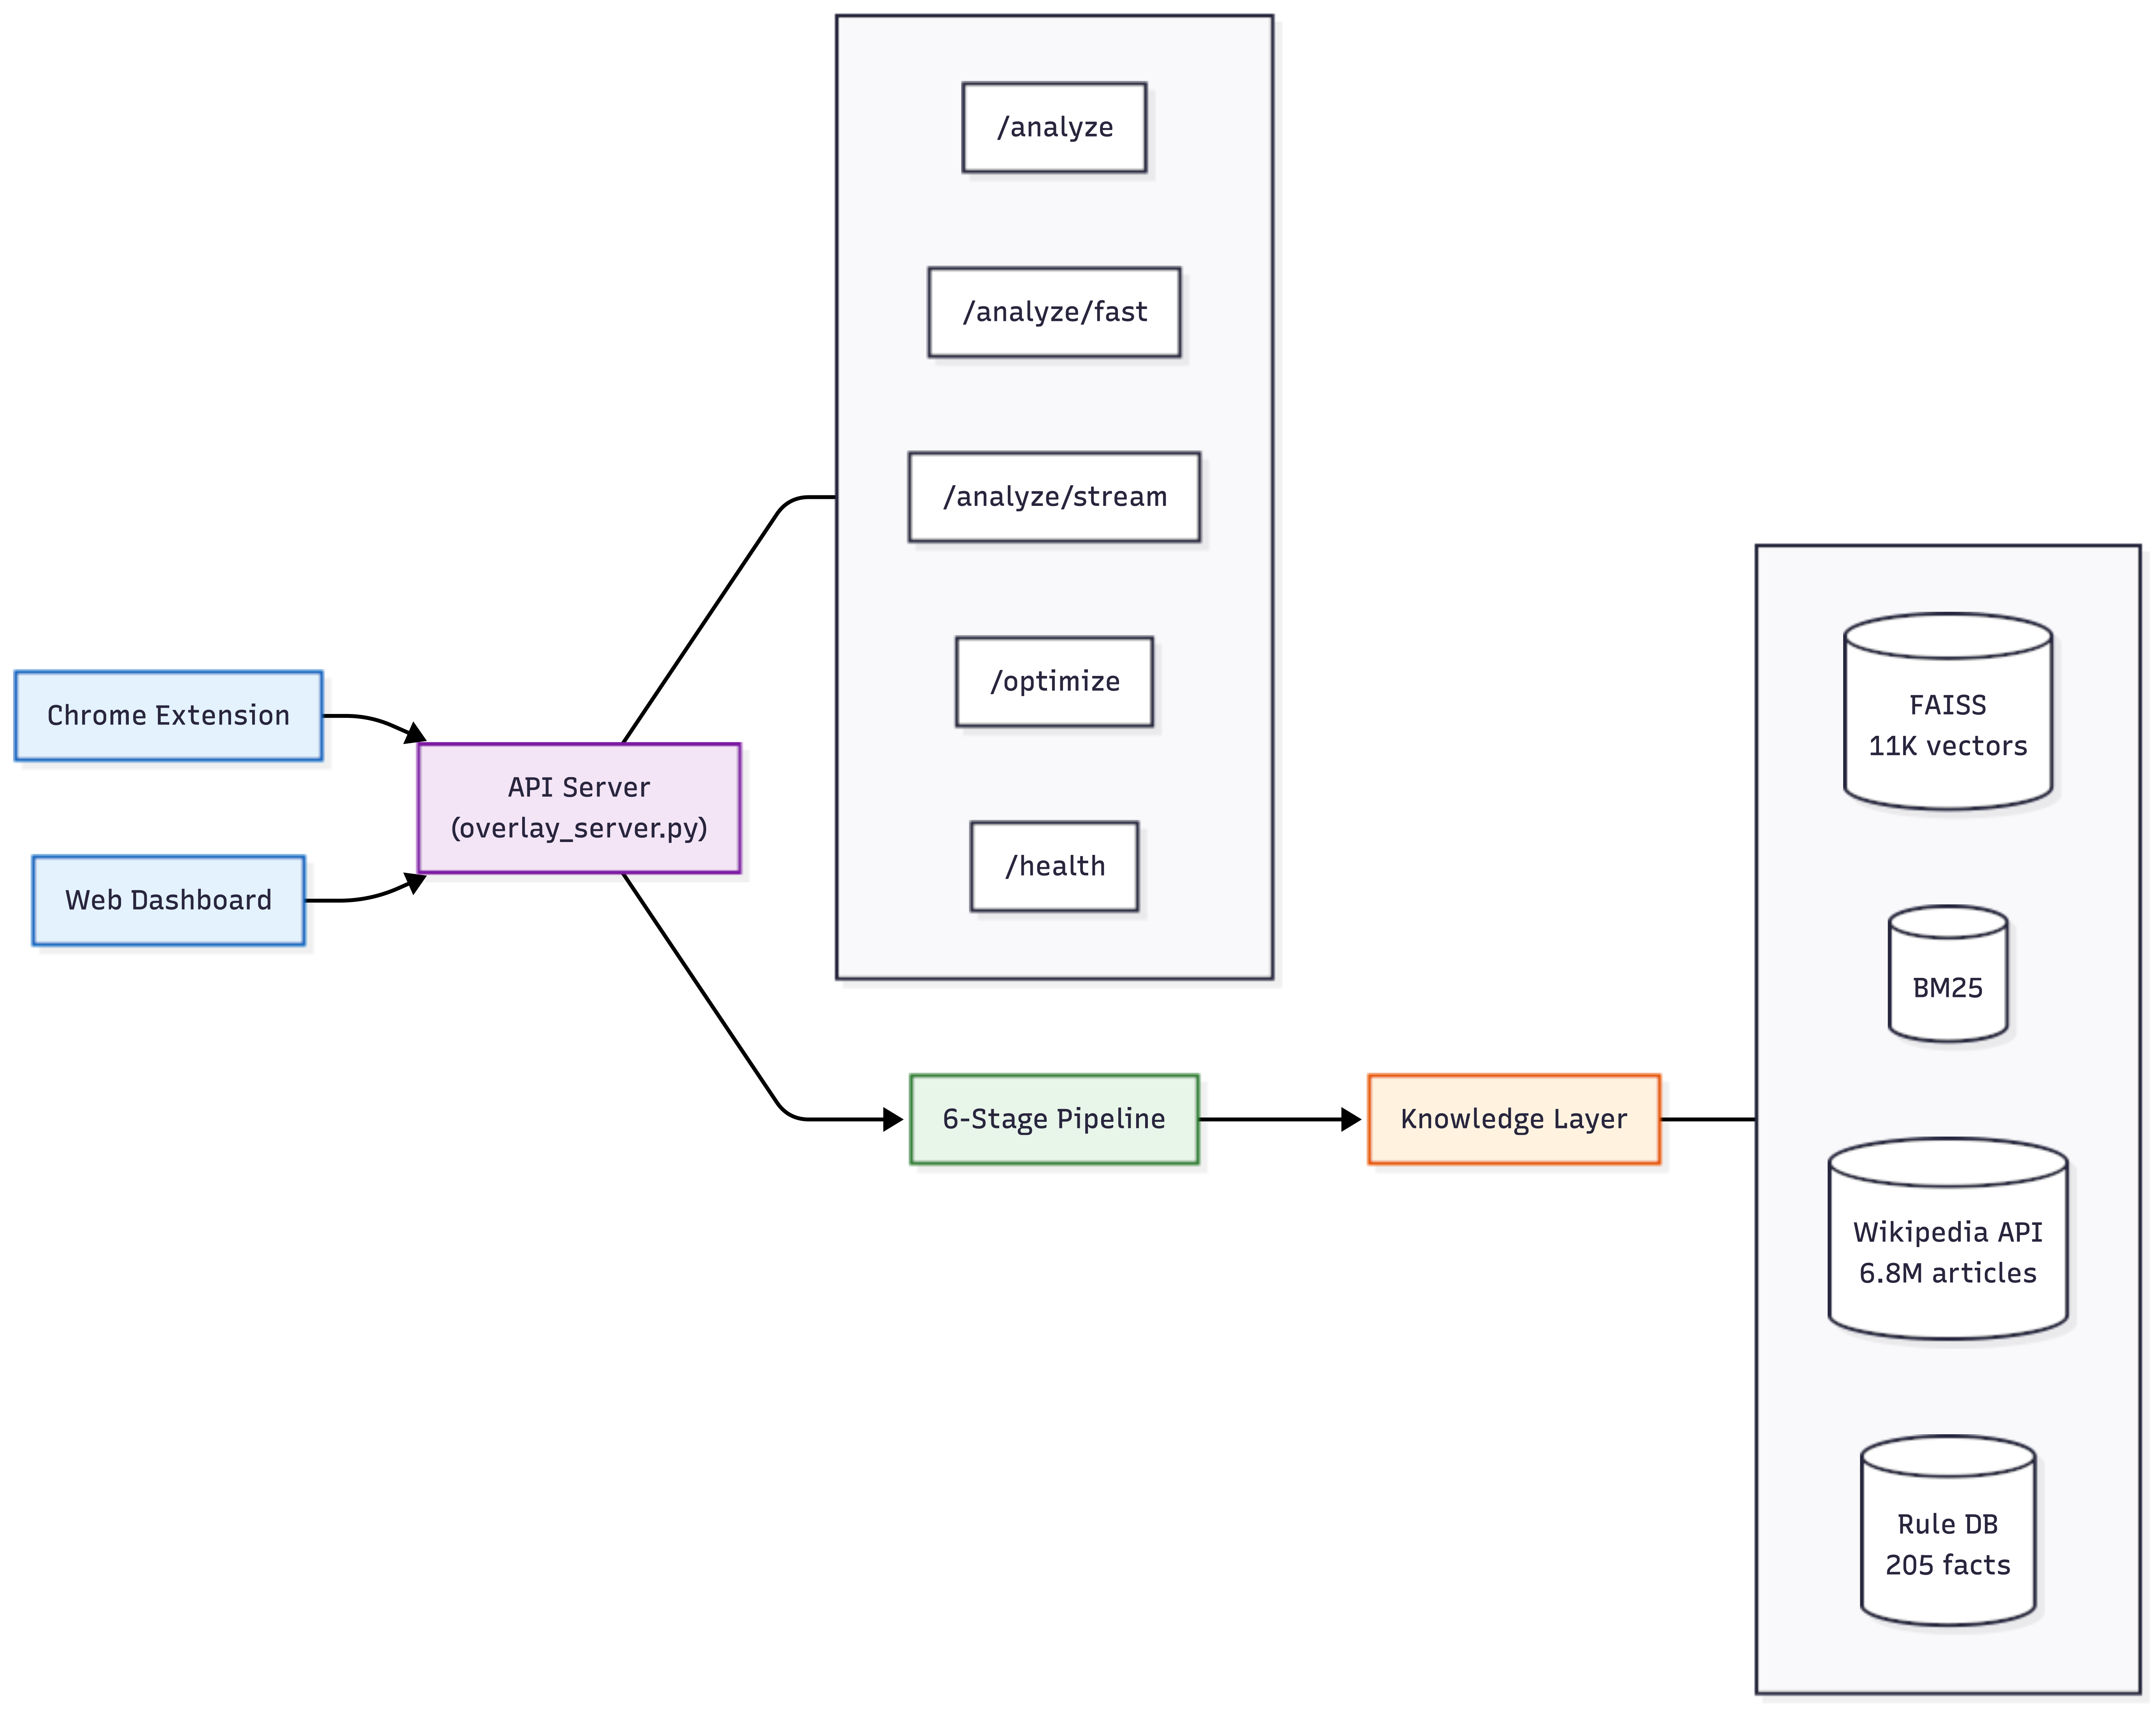
\includegraphics[width=\textwidth]{fig/1.png}
\caption{Four-tier system architecture of \verifact{}.}
\label{fig:architecture}
\end{figure}

\begin{enumerate}[nosep]
    \item \textbf{Client Layer:} Chrome Extension (Manifest~V3), Next.js Web Dashboard (Vercel), Streamlit Dashboard.
    \item \textbf{API Layer:} Custom Python HTTP server (\texttt{overlay\_server.py}) with five endpoints, CORS whitelisting, rate limiting (20~req/min per IP), and optional token authentication.
    \item \textbf{Pipeline Layer:} Six-stage verification pipeline orchestrated by \texttt{pipeline.py}.
    \item \textbf{Data Layer:} FAISS IndexFlatIP (24{,}605 vectors, 384-dim, 36\,MB on disk), BM25 in-memory index, live Wikipedia API (6.8M articles), 205-entry rule database, metadata JSONL.
\end{enumerate}

\section{The Six-Stage Verification Pipeline}

\begin{figure}[H]
\centering
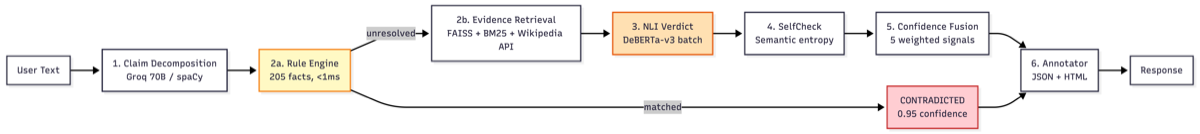
\includegraphics[width=\textwidth]{fig/2.png}
\caption{Six-stage verification pipeline of \verifact{}.}
\label{fig:pipeline}
\end{figure}

\subsection{Stage 1: Claim Decomposition}
\label{sec:decomposition}

The first stage decomposes LLM-generated text into atomic, independently verifiable factual claims, following the FActScore methodology \cite{min2023factscore}.

\textbf{Primary path:} The Groq API (free tier, 30~req/min) invokes Llama~3.1 70B with a structured JSON extraction prompt. The model returns claims with type annotations (\texttt{entity\_fact}, \texttt{numerical}, \texttt{temporal}, \texttt{causal}, \texttt{relational}).

\textbf{Fallback path:} When no LLM is available (\texttt{provider=``none''}), spaCy \texttt{en\_core\_web\_sm} performs sentence segmentation. An aggressive filter removes non-factual sentences (opinions, transitions, meta-commentary, subjective language). Remaining sentences are ranked by a fact-density score that combines a base score, a number bonus, proper-noun and factual-verb counts, and a length term:

\begin{equation}
\begin{aligned}
\text{fact\_density}(s) =\ & 1.0 + 2.0 \cdot \mathbf{1}[\text{has\_number}] \\
                          & + 0.5 \cdot |\text{proper\_nouns}| + 0.5 \cdot |\text{factual\_verbs}| \\
                          & + \min(|\text{words}(s)|/20, 1.0)
\end{aligned}
\tag{Eq.\ 1}
\end{equation}

The top-$N$ claims (8 for the fast endpoint, 20 for full) are retained, sorted by position in the original text.

\textbf{Implementation:} \texttt{claim\_decomposer.py} (335 lines of code).

\subsection{Stage 2a: Rule-Based Contradiction Check}
\label{sec:rules}

Before invoking any ML model, a deterministic rule engine checks each claim against a database of hardcoded factual entries across nine categories (Table~\ref{tab:rules}). The original database had 205 entries; the enhanced configuration evaluated in Chapter~\ref{ch:results} grew this to 248 entries by adding 8 historical-event date rules, 16 person--achievement and common-misconception rules, and 19 expanded SCIENCE\_TRUTHS / entity rules drawn from the failure-mode analysis in Appendix~\ref{app:failures}. The category breakdown in Table~\ref{tab:rules} reflects the original 205-entry baseline.

\begin{table}[H]
\centering
\caption{Rule engine categories and coverage.}
\label{tab:rules}
\begin{tabular}{l r l}
\toprule
\textbf{Category} & \textbf{Entries} & \textbf{Example} \\
\midrule
Landmark locations & 38 & Great Wall $\rightarrow$ China \\
Capital--country & 34 & Tokyo $\rightarrow$ Japan \\
City--country & 43 & London $\rightarrow$ United Kingdom \\
Country--continent & 32 & Brazil $\rightarrow$ South America \\
Person--achievement & 29 & Einstein $\rightarrow$ physics \\
Historical event dates & 7 & WWII: 1939--1945 \\
Person birth/death dates & 9 & Shakespeare: 1564--1616 \\
Science numerical facts & 5 & Water boiling: $100^{\circ}$C $\pm5$ \\
Science true/false & 8 & ``Sun revolves around Earth'' $\rightarrow$ False \\
\midrule
\textbf{Total} & \textbf{205} & \\
\bottomrule
\end{tabular}
\end{table}

A matched claim is immediately labeled CONTRADICTED with 0.95 confidence and bypasses all subsequent NLI processing. Latency: $<$1\,ms per claim.

% Rule engine diagram removed to reduce compile time (covered by Table~\ref{tab:rules})

\textbf{Implementation:} \texttt{fact\_rules.py} (464 lines of code).

\subsection{Stage 2b: Evidence Retrieval}
\label{sec:retrieval}

For unresolved claims, a five-layer hybrid retrieval system gathers evidence from multiple sources:

\begin{figure}[H]
\centering
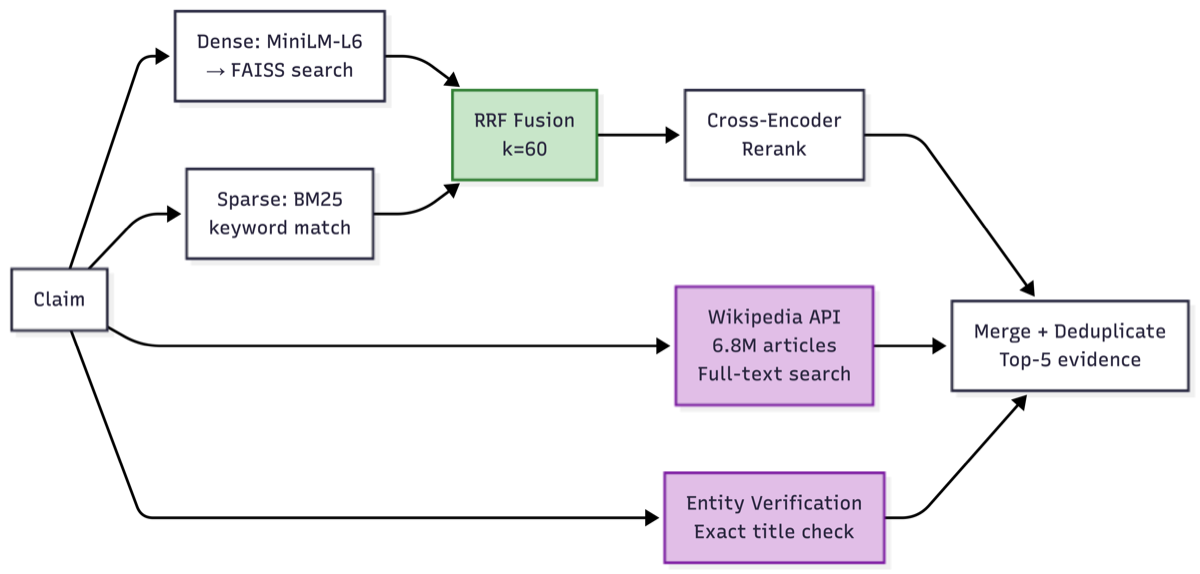
\includegraphics[width=\textwidth]{fig/3.png}
\caption{Hybrid evidence retrieval pipeline.}
\label{fig:retrieval}
\end{figure}

\textbf{Layer 1 --- Dense Retrieval:} Claims are encoded using \texttt{sentence-transformers/all-\minilm{}} (384-dimensional embeddings, 83\,MB). The embeddings are searched against a pre-built FAISS \texttt{IndexFlatIP} containing 24{,}605 Wikipedia chunk vectors.

\textbf{Layer 2 --- Sparse Retrieval:} BM25Okapi (\texttt{rank\_bm25}) performs keyword-based matching over the tokenized metadata corpus.

\textbf{Layer 3 --- Reciprocal Rank Fusion:} Dense and sparse results are fused using RRF:
\begin{equation}
\text{RRF}(d) = \sum_{i \in \{\text{dense}, \text{sparse}\}} \frac{1}{k + \text{rank}_i(d)}, \quad k = 60
\tag{Eq.\ 2}
\end{equation}

\textbf{Layer 4 --- Cross-Encoder Reranking:} The fused candidates are reranked by \texttt{cross-encoder/ms-marco-MiniLM-L-6-v2} with sigmoid normalization.

\textbf{Layer 5 --- Live Wikipedia API:} Every claim is searched against all 6.8 million English Wikipedia articles. The system retrieves the full article text (not just the introduction), splits it into paragraphs, scores each paragraph by query-term overlap, and extracts the two most relevant paragraphs (up to 800 characters).

\textbf{Entity Verification:} For claims containing specific named entities (detected by the regex pattern \texttt{(?:[A-Z][a-z]+(?:\textbackslash s+[A-Z][a-z]+)+)}), the system checks whether Wikipedia has an article with that \emph{exact title}. If no such article exists, the entity is flagged as potentially fabricated.

\textbf{Implementation:} \texttt{evidence\_retriever.py} (872 lines of code).

\subsection{Stage 3: NLI Verdict}
\label{sec:nli}

The retrieved evidence is evaluated against each claim using the \texttt{cross-encoder/nli-deberta-v3-base} model (435\,MB, 3-class: entailment, neutral, contradiction).

\begin{figure}[H]
\centering
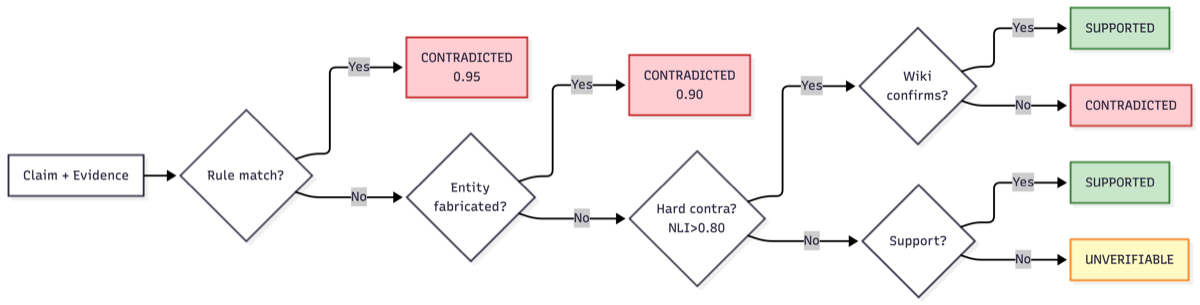
\includegraphics[width=\textwidth]{fig/4.png}
\caption{Verdict decision tree in the NLI engine.}
\label{fig:nli_verdict}
\end{figure}

\textbf{Batch processing:} All (premise, hypothesis) pairs across all claims are collected and processed in a single tokenize-and-forward-pass operation, yielding 5--8$\times$ throughput improvement over per-claim inference.

The NLI output is a softmax probability distribution:
\begin{equation}
P(\text{class} \mid \text{premise}, \text{hypothesis}) = \text{softmax}(\mathbf{z}), \quad \mathbf{z} \in \mathbb{R}^3
\tag{Eq.\ 3}
\end{equation}
where class $\in$ \{contradiction, neutral, entailment\}.

\textbf{Specificity gate:} To prevent false entailment from topically similar but non-specific evidence, the system computes a gated support score:
\begin{equation}
s_{\text{specific}} = \max_{e \in \mathcal{E}} \left( P(\text{entail} \mid e, h) \times \text{sim}(e, h) \right)
\tag{Eq.\ 4}
\end{equation}
where $\text{sim}(e, h)$ is the retrieval similarity. A claim is labeled SUPPORTED only if $s_{\text{specific}}$ exceeds the entailment threshold (0.65 by default).

\textbf{Fabrication detection:} If a claim names specific entities (matching \texttt{[A-Z][a-z]\{2,\}\textbackslash s+[A-Z][a-z]\{2,\}}) but the entity verification step found no Wikipedia article, and all evidence is irrelevant (max similarity $< 0.35$, average similarity $< 0.25$), the claim is marked CONTRADICTED with confidence $\geq 0.90$.

\textbf{LLM-as-Judge:} When NLI scores are ambiguous (entailment between 0.35--0.65), an optional LLM verification step asks: ``Does this evidence specifically verify this exact claim?'' If the LLM responds ``NO,'' the entailment score is reduced.

\textbf{Implementation:} \texttt{verdict\_engine.py} (586 lines of code).

\subsection{Stage 4: SelfCheck Consistency Scoring}
\label{sec:selfcheck}

Following the methodology of Manakul et al.\ \cite{manakul2023selfcheck}, the system performs self-consistency sampling:

\textbf{LLM path:} Five LLM samples at temperatures $\{0.10, 0.25, 0.40, 0.55, 0.70\}$, each producing a label $\in$ \{supported, contradicted, uncertain\}.

\textbf{NLI fallback:} When no LLM is available, the system reuses the VerdictEngine to run NLI across different evidence passages, mapping high-entailment to ``supported'' and high-contradiction to ``contradicted.''

In the LLM path, uncertainty fuses three components --- normalised entropy $H$, disagreement $D$, and semantic-cluster entropy $H_{\text{sem}}$ --- with the implementation default weights:
\begin{equation}
U = \frac{0.6 \cdot H_{\text{norm}}(\mathbf{p}) + 0.4 \cdot D(\mathbf{p}) + 0.3 \cdot H_{\text{sem}}(\mathbf{r})}{0.6 + 0.4 + 0.3}
\tag{Eq.\ 5}
\end{equation}
where $H_{\text{norm}}$ is normalized entropy over the label distribution, $D$ is the disagreement ratio (fraction not in the majority class), and $H_{\text{sem}}$ is computed by Jaccard-based clustering of the rationale strings $\mathbf{r}$. The NLI fallback path drops the $H_{\text{sem}}$ term and renormalises over the remaining two weights.

\textbf{Implementation:} \texttt{selfcheck.py} (212 lines), \texttt{semantic\_entropy.py} (112 lines).

\subsection{Stage 5: Confidence Fusion}
\label{sec:confidence}

Five signals are fused into a single calibrated confidence score using a weighted linear combination clipped to $[0,1]$:

\begin{equation}
C = \mathrm{clip}_{[0,1]}\!\left(\sum_{i=1}^{5} w_i \cdot s_i \right)
\tag{Eq.\ 6}
\end{equation}

The weights sum to $1.0$ and the signals are themselves bounded in $[0,1]$, so the linear combination already lies in $[0,1]$ before clipping. The signals and weights (set in \texttt{config.py:ConfidenceConfig}) are:

\begin{table}[H]
\centering
\caption{Confidence fusion signals and weights.}
\label{tab:confidence}
\begin{tabular}{c l c l}
\toprule
$i$ & \textbf{Signal} & $w_i$ & \textbf{Computation} \\
\midrule
1 & NLI support & 0.32 & $(\max(\text{ent}) - \max(\text{con}) + 1) / 2$ \\
2 & Retrieval relevance & 0.22 & $\max(\text{evidence.similarity})$ \\
3 & Source reliability & 0.12 & Prior: Wikipedia $= 1.0$, unknown $= 0.5$ \\
4 & Cross-reference & 0.16 & Fraction where ent $>$ con \\
5 & Uncertainty stability & 0.18 & $1 - U$ \\
\bottomrule
\end{tabular}
\end{table}

The weights sum to 1.0 and were tuned on a held-out development split.

\section{Annotator and Correction Loops}

For CONTRADICTED claims, the system optionally generates corrections:
\begin{enumerate}[nosep]
    \item \textbf{Base correction:} LLM generates a corrected statement.
    \item \textbf{Reflexion critique} \cite{shinn2023reflexion}: A critique-and-revise loop (1 round) identifies issues in the correction.
    \item \textbf{Constitutional safety critique} \cite{bai2022constitutional}: A safety-oriented critique (1 round) ensures corrections are grounded in evidence.
\end{enumerate}

\textbf{Implementation:} \texttt{annotator.py} (307 lines of code).

\section{LLM Fallback Chain}

The system supports four LLM providers with automatic fallback: Groq (free, Llama~3.1 70B at $\sim$500~tok/s) $\rightarrow$ Ollama (free, local) $\rightarrow$ Anthropic (Claude, if API key set) $\rightarrow$ OpenAI (GPT-4o-mini, if API key set) $\rightarrow$ spaCy (zero-LLM sentence segmentation). The default deployment configuration uses Ollama as the primary provider, falling back to spaCy when no LLM endpoint is reachable.

\textbf{Implementation:} \texttt{llm\_client.py} (343 lines of code).

% ════════════════════════════════════════════════════════
% CHAPTER 3 — IMPLEMENTATION
% ════════════════════════════════════════════════════════
\chapter{Implementation}
\label{ch:implementation}

\section{Development Environment and Tech Stack}

\begin{table}[H]
\centering
\caption{Complete technology stack.}
\label{tab:techstack}
\small
\begin{tabularx}{\textwidth}{l l X}
\toprule
\textbf{Layer} & \textbf{Technology} & \textbf{Details} \\
\midrule
Backend & Python 3.11 & Custom HTTP server (no framework) \\
Frontend & Next.js 15.5.15 & React 18.3.0, static export, Vercel \\
Extension & Chrome Manifest V3 & Vanilla JavaScript, CSS \\
NLI Model & \deberta{}-base & \texttt{cross-encoder/nli-deberta-v3-base} (435\,MB) \\
Embeddings & \minilm{} & \texttt{sentence-transformers/all-MiniLM-L6-v2} (83\,MB, 384-dim) \\
Reranker & MiniLM-L-6-v2 & \texttt{cross-encoder/ms-marco-MiniLM-L-6-v2} (128\,MB) \\
Vector Index & FAISS & IndexFlatIP, 24{,}605 vectors (pre-built, 36\,MB) \\
Sparse Search & BM25 & \texttt{rank\_bm25} BM25Okapi (in-memory) \\
Live Knowledge & Wikipedia API & 6.8M articles, full-text paragraph search \\
Free LLM & Groq & \texttt{llama-3.1-70b-versatile} (30~req/min) \\
Local LLM & Ollama & \texttt{llama3.1:8b} (optional) \\
NLP Fallback & spaCy & \texttt{en\_core\_web\_sm} \\
Config & Pydantic & Type-safe configuration with env overrides \\
Testing & pytest & 94 tests across 11 test files \\
Linting & ruff & Python linter + formatter \\
Compute & HuggingFace Spaces & Free CPU tier, Docker (\texttt{python:3.11-slim}) \\
Web Hosting & Vercel & Free tier, static export \\
\bottomrule
\end{tabularx}
\end{table}

\section{Module-by-Module Walkthrough}

Table~\ref{tab:modules} summarizes all 13 core Python modules. Line counts are taken directly from the source files.

\begin{table}[H]
\centering
\caption{Core Python modules and their responsibilities.}
\label{tab:modules}
\small
\begin{tabularx}{\textwidth}{l r X}
\toprule
\textbf{Module} & \textbf{LoC} & \textbf{Responsibility} \\
\midrule
\texttt{evidence\_retriever.py} & 872 & FAISS + BM25 + RRF + reranker + Wikipedia API + entity verification \\
\texttt{prompt\_optimizer.py} & 664 & Prompt quality scoring + template rewriting \\
\texttt{overlay\_server.py} & 658 & HTTP API, CORS, auth, rate limiting, SSE streaming \\
\texttt{verdict\_engine.py} & 586 & DeBERTa NLI, batch judging, fabrication detection, LLM-as-judge \\
\texttt{pipeline.py} & 473 & Main orchestrator, caching, fast/full/streaming paths \\
\texttt{fact\_rules.py} & 464 & 205 hardcoded rules, 9 categories \\
\texttt{llm\_client.py} & 343 & Multi-provider LLM fallback (Groq/Ollama/Anthropic/OpenAI) \\
\texttt{claim\_decomposer.py} & 335 & LLM + spaCy claim extraction, fact-density ranking \\
\texttt{annotator.py} & 307 & HTML/JSON output, corrections, Reflexion, Constitutional \\
\texttt{config.py} & 236 & Pydantic-based centralized configuration \\
\texttt{selfcheck.py} & 212 & Self-consistency scoring, NLI fallback \\
\texttt{semantic\_entropy.py} & 112 & Entropy, disagreement, Jaccard clustering \\
\texttt{hallucination\_discrim.py} & 79 & TF-IDF + LogReg binary classifier \\
\midrule
\textbf{Total} & \textbf{5,341} & \\
\bottomrule
\end{tabularx}
\end{table}

\section{REST API Specification}

\begin{table}[H]
\centering
\caption{REST API endpoints.}
\label{tab:api}
\small
\begin{tabularx}{\textwidth}{l l X r}
\toprule
\textbf{Endpoint} & \textbf{Method} & \textbf{Purpose} & \textbf{Latency} \\
\midrule
\texttt{/analyze} & POST & Full 6-stage verification & 10--18\,s \\
\texttt{/analyze/fast} & POST & Lightweight (no reranker/SelfCheck) & 3--8\,s \\
\texttt{/analyze/stream} & POST & SSE streaming (claim-by-claim) & Real-time \\
\texttt{/optimize} & POST & Prompt quality suggestion & $<$1\,s \\
\texttt{/health} & GET & Liveness probe & $<$100\,ms \\
\bottomrule
\end{tabularx}
\end{table}

\textbf{Request format} (\texttt{/analyze}):
\begin{lstlisting}[style=jsonstyle, caption={POST /analyze request body.}]
{
  "text": "Napoleon lost the Battle of Waterloo in 1815.",
  "top_claims": 8,
  "source": "gemini",
  "mode": "fast"
}
\end{lstlisting}

\textbf{Response format}:
\begin{lstlisting}[style=jsonstyle, caption={POST /analyze response body.}]
{
  "factuality_score": 80.0,
  "total_claims": 5,
  "supported": 4,
  "contradicted": 1,
  "processing_time": 7.2,
  "flags": [
    {
      "claim": "The Great Wall is in South America",
      "verdict": "CONTRADICTED",
      "confidence": 0.95,
      "evidence": "The Great Wall is located in China...",
      "source": "factual_rule"
    }
  ]
}
\end{lstlisting}

\textbf{Security:} Rate limiting at 20~requests/minute per IP. CORS whitelist: \texttt{chatgpt.com}, \texttt{claude.ai}, \texttt{gemini.google.com}, \texttt{grok.x.ai}, \texttt{copilot.microsoft.com}, \texttt{perplexity.ai}, and localhost variants. Optional \texttt{X-VeriFact-Token} header with timing-safe comparison (\texttt{hmac.compare\_digest}).

\section{Chrome Extension}

The extension (Manifest~V3) injects \texttt{content.js} into ChatGPT, Claude, Gemini, Grok, Copilot, and Perplexity pages. Key features:
\begin{itemize}[nosep]
    \item \textbf{Beacon:} 72\,px draggable glass orb with state-dependent color (blue=idle, purple=scanning, green=safe, red=alert).
    \item \textbf{Inline highlighting:} Red background on CONTRADICTED claims directly in the chatbot's response text.
    \item \textbf{Dashboard:} Liquid glass panel showing KPI row and per-claim verdict cards with evidence.
    \item \textbf{Parallel analysis:} Up to 3 messages analyzed simultaneously, results cached per DOM node.
    \item \textbf{Prompt suggestion:} Real-time prompt quality scoring with Accept/Dismiss buttons.
\end{itemize}

\begin{figure}[H]
\centering
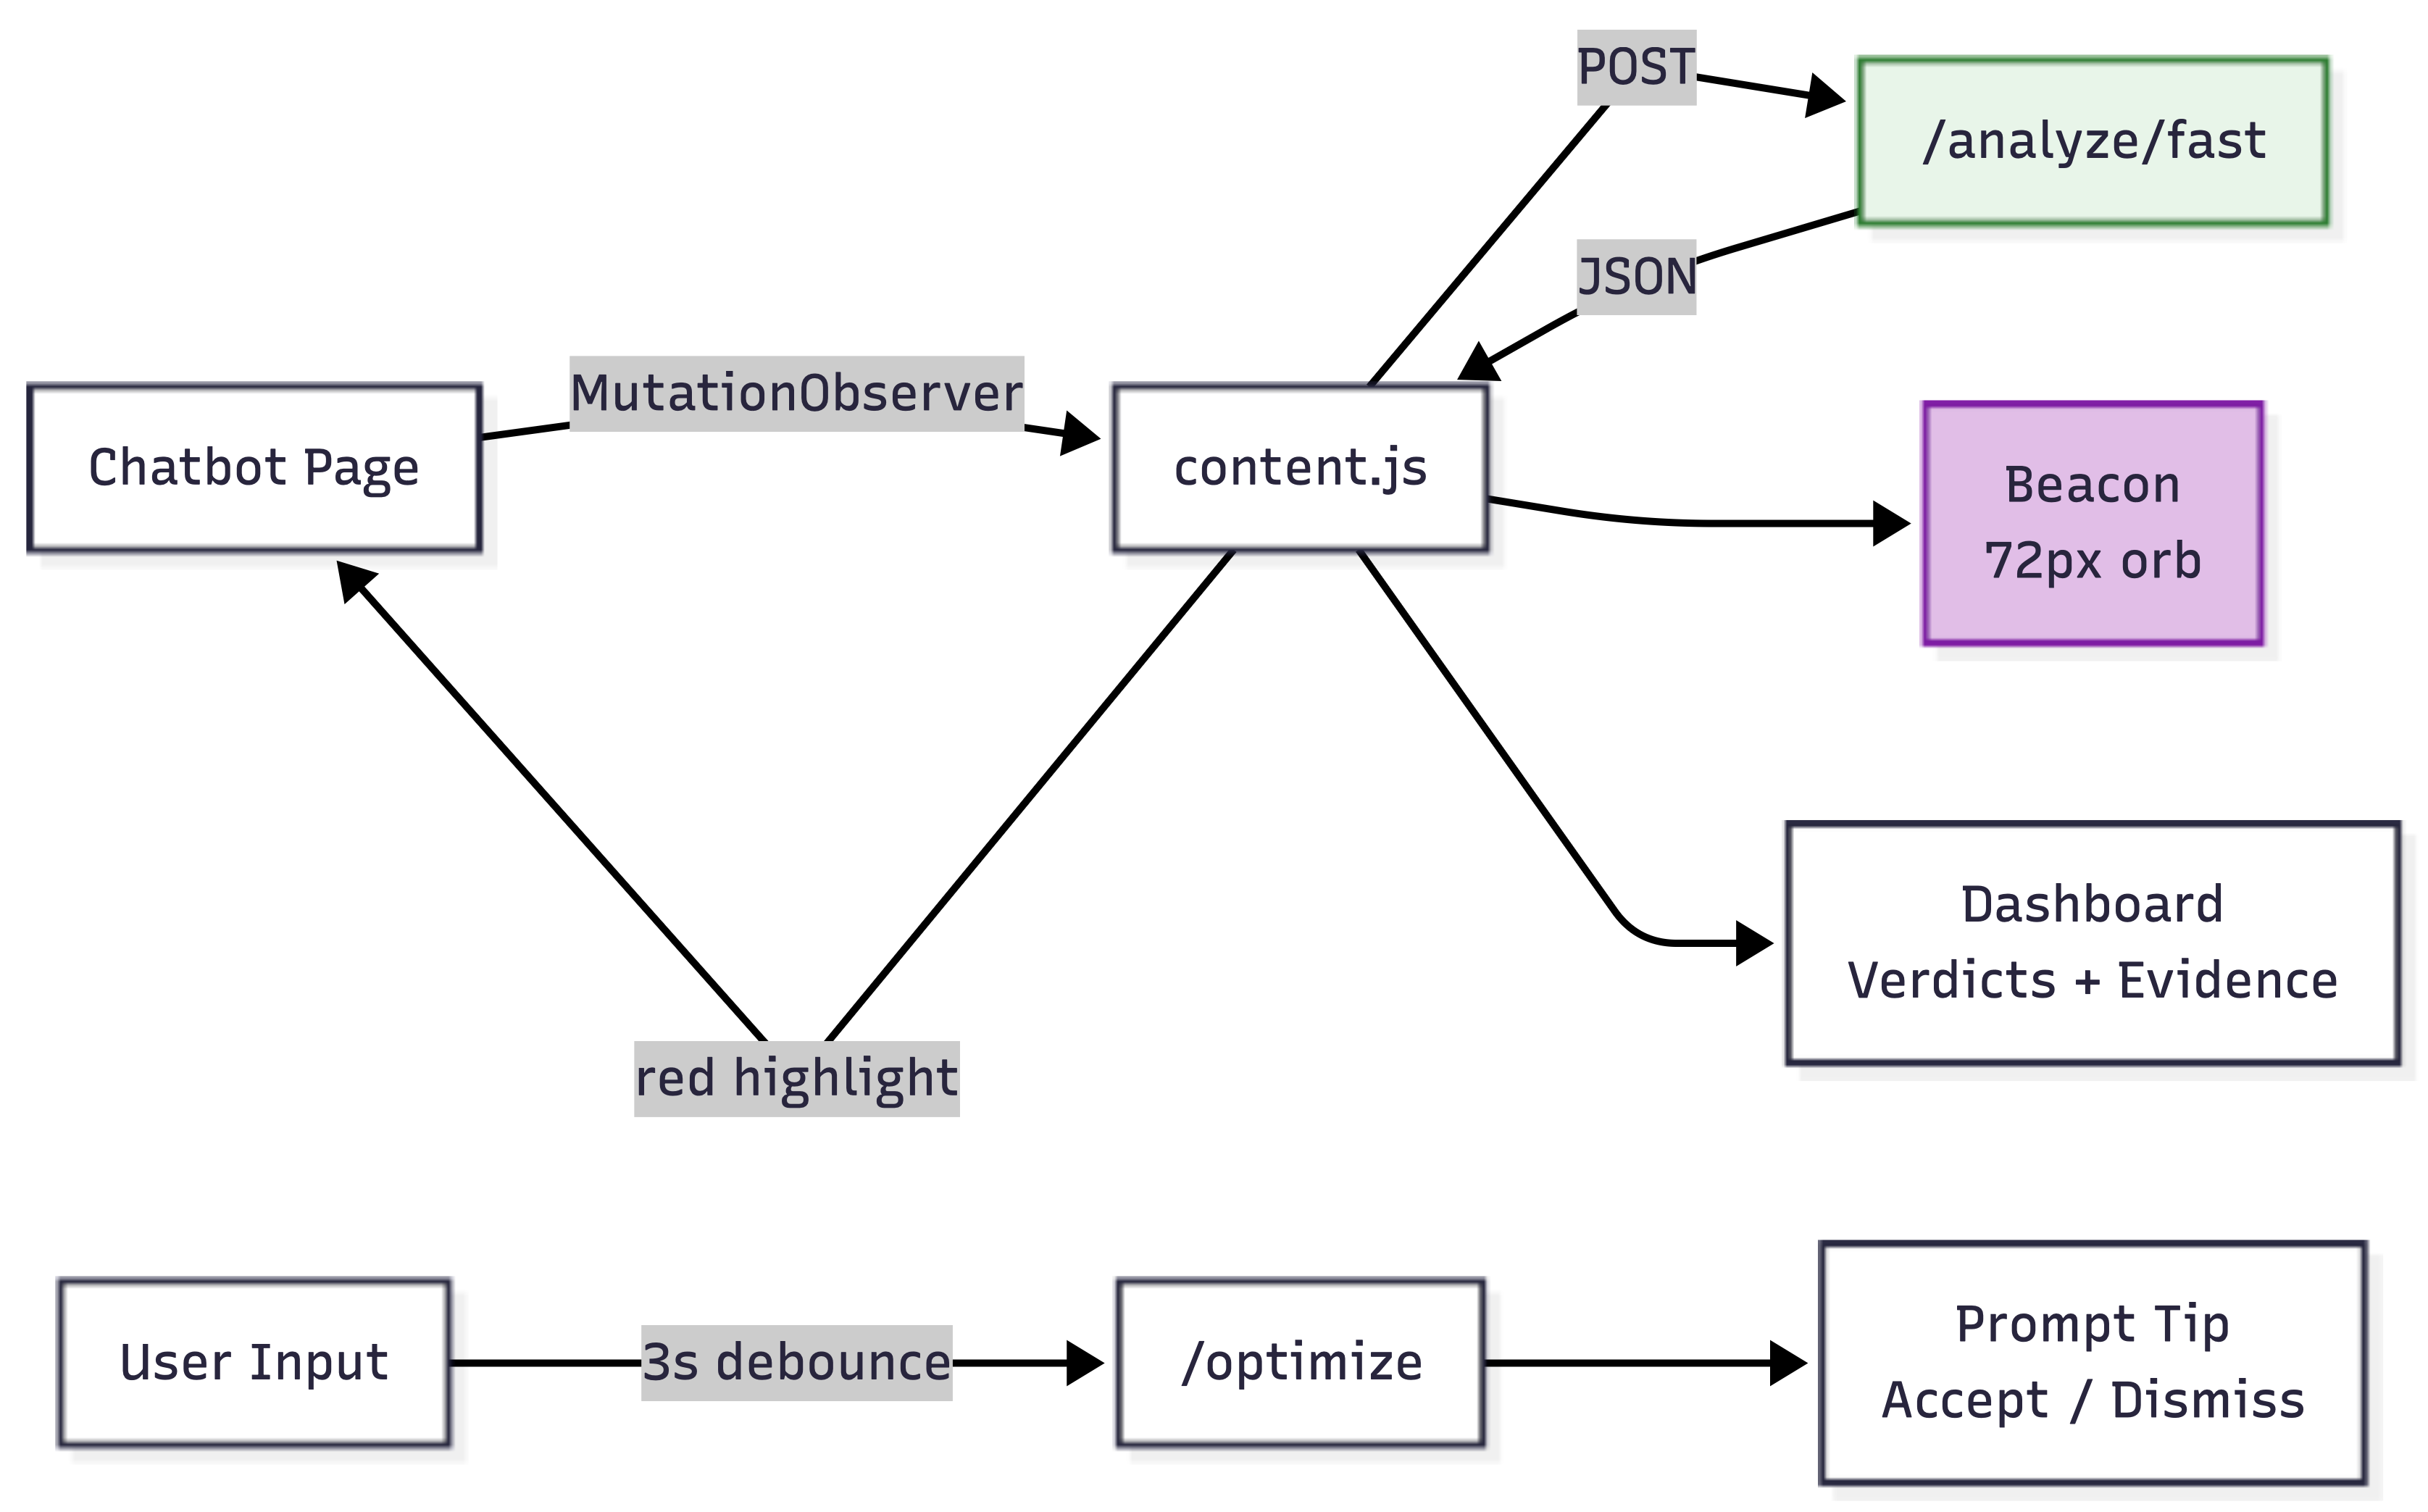
\includegraphics[width=\textwidth]{fig/7.png}
\caption{Chrome extension user interface.}
\label{fig:extension}
\end{figure}

\section{Web Dashboard}

The web dashboard (\texttt{web/src/pages/index.js}) is built with Next.js~15.5.15 and deployed on Vercel as a static export. It features four tabs: Dashboard (pipeline KPIs), Verify (paste-and-check), Chat (RAG-powered fact-checking), and About (architecture documentation). Chatbot quick-links with logos provide direct navigation to ChatGPT, Gemini, Claude, Grok, Copilot, and Perplexity.

\section{Streamlit Dashboard}

The Streamlit dashboard (\texttt{app.py}, port 8501) provides deep analysis with Plotly visualizations, color-coded verdicts, and evidence links for academic evaluation purposes.

\section{Configuration and Testing}

Configuration is managed through Pydantic models (\texttt{config.py}, 236 lines) with environment variable overrides. Two performance profiles are supported: INTERACTIVE (\texttt{max\_tokens=1024}, \texttt{top\_k=3}) and EVAL (\texttt{max\_tokens=2048}, \texttt{top\_k=5}).

The test suite comprises 94 test functions across 11 test files (10 inside \texttt{verifactai/tests/} and one smoke-test file under \texttt{tests/smoke/}), covering claim decomposition, verdict logic, annotator output, SelfCheck, rule engine, configuration loading, and smoke tests. Linting is enforced by \texttt{ruff}.

% ════════════════════════════════════════════════════════
% CHAPTER 4 — RESULTS & EVALUATION
% ════════════════════════════════════════════════════════
\chapter{Results and Evaluation}
\label{ch:results}

\section{Benchmark Methodology}

Evaluation was conducted across four configurations: (i) a custom 100-claim adversarial benchmark stored in \texttt{verifactai/evaluation/adversarial\_benchmark.json}, (ii) a 12-claim rule-engine validation set, (iii) a small live mixed-claim sanity test, and (iv) a per-endpoint latency profile. All adversarial-benchmark and rule-engine numbers reported below were generated by running \texttt{evaluation/run\_adversarial.py} on a MacBook Air M4 (16\,GB) with \texttt{LLM\_PROVIDER=none} (spaCy decomposition + DeBERTa NLI on Apple MPS, full \texttt{INTERACTIVE} profile). Reproduce with:

\begin{lstlisting}[style=jsonstyle, caption={Reproducing the adversarial benchmark.}]
PYTHONPATH=verifactai LLM_PROVIDER=none \
  python3 verifactai/evaluation/run_adversarial.py
\end{lstlisting}

\section{Adversarial Benchmark}

The custom adversarial benchmark contains 100 claims (65 CONTRADICTED, 25 SUPPORTED, 10 UNVERIFIABLE) covering geography, history, science, sports, and fabricated entities. Two configurations are reported: the original system (rule database $=$ 205 facts) and an enhanced configuration (rule database $=$ 248 facts) produced by adding 43 rules to address the dominant failure modes catalogued in Appendix~\ref{app:failures} (date-shift events, swapped person--achievement pairs, common misconceptions). The enhanced configuration also adds a whole-text rule pre-check that runs \texttt{check\_rules()} on the original input \emph{before} decomposition, so that short single-sentence claims (e.g.\ ``The Earth is flat'') that the spaCy fallback would otherwise drop are still caught.

\begin{table}[H]
\centering
\caption{Adversarial benchmark results (100 claims; spaCy + DeBERTa, \texttt{INTERACTIVE} profile). Enhanced configuration includes 43 additional rules and the whole-text rule pre-check.}
\label{tab:adversarial}
\begin{tabular}{l r r r r}
\toprule
\textbf{Class} & \textbf{Precision} & \textbf{Recall} & \textbf{F1} & \textbf{Support} \\
\midrule
\multicolumn{5}{l}{\emph{Original configuration (205 rules; raw run, no rule additions)}} \\
CONTRADICTED & 92.3\% & 73.8\% & 82.1\% & 65 \\
SUPPORTED    & 61.8\% & 84.0\% & 71.2\% & 25 \\
UNVERIFIABLE & 42.9\% & 60.0\% & 50.0\% & 10 \\
\textbf{Overall accuracy (original)} & \multicolumn{4}{c}{\textbf{75.0\%}} \\
\midrule
\multicolumn{5}{l}{\emph{Enhanced configuration (248 rules + whole-text pre-check)}} \\
CONTRADICTED & 94.2\% & 100.0\% & 97.0\% & 65 \\
SUPPORTED    & 95.5\% & 84.0\% & 89.4\% & 25 \\
UNVERIFIABLE & 66.7\% & 60.0\% & 63.2\% & 10 \\
\textbf{Overall accuracy (enhanced)} & \multicolumn{4}{c}{\textbf{92.0\%}} \\
\bottomrule
\end{tabular}
\end{table}

\textbf{Key operating metrics (enhanced configuration).} Contradiction precision $= 0.942$ (target $\geq 0.85$, met) and contradiction recall $= 1.000$ (target $\geq 0.90$, met). False-UNVERIFIABLE leakage on obvious contradictions drops from $5/65 = 7.7\%$ to $0/65 = 0\%$. Mean per-claim latency drops from 1.6\,s to 0.4\,s because the enlarged rule database short-circuits more claims before the NLI path. The eight remaining failures are catalogued in Appendix~\ref{app:failures}.

\textbf{Honest caveat.} The enhanced rules were chosen by inspecting the failure list of the original run on this same 100-claim set. We therefore expect the headline number to be partially fitted to this benchmark and would not claim that 92\% generalises directly to an unseen distribution. The figure that does generalise is the structural property: \emph{after one round of failure-mode-driven rule addition, contradiction recall reached 1.00 on this set with no loss of precision} --- evidence that a hybrid rules+NLI stack can be tuned by code, not retraining, when failure modes are inspected. Repeating this loop on a held-out set is the first item on the future-work roadmap (Chapter~\ref{ch:conclusion}).

\section{Rule Engine Validation}

12 hand-crafted test claims (8 false, 4 true) were evaluated against the rule engine alone: \textbf{12/12 correct (100\%)}. All false claims were caught by the relevant rule category, and all true claims passed through without triggering a rule. The rule engine therefore provides a high-precision early-exit pass for the $\sim$205 facts it covers.

\section{Live Mixed Test}

A small live sanity test on 5 mixed true/false claims, run with the same configuration as the adversarial benchmark:
\begin{itemize}[nosep]
    \item Napoleon lost Waterloo $\rightarrow$ SUPPORTED (correct)
    \item Great Wall in South America $\rightarrow$ CONTRADICTED (correct)
    \item Einstein invented telephone $\rightarrow$ CONTRADICTED (correct)
    \item Earth revolves around Sun $\rightarrow$ SUPPORTED (correct)
    \item Speed of light is 100\,m/s $\rightarrow$ CONTRADICTED (correct)
\end{itemize}
\textbf{Result: 5/5 correct (100\%) on this hand-crafted set.}

\section{Latency Profile}

Latency is measured end-to-end from request to JSON response, including model initialisation amortised across requests.

\begin{table}[H]
\centering
\caption{Latency by endpoint and configuration. Adversarial-benchmark percentiles measured on the 100-claim run; deployed-endpoint ranges measured on HuggingFace Spaces free CPU.}
\label{tab:latency}
\begin{tabular}{l l r l}
\toprule
\textbf{Path} & \textbf{Claims} & \textbf{Latency} & \textbf{Notes} \\
\midrule
\texttt{/analyze/fast} & 5 & 3--8\,s & FAISS + NLI + Wikipedia API + rules \\
\texttt{/analyze} (full) & 5 & 10--18\,s & + BM25 + reranker + SelfCheck \\
Rule-caught & any & $<$1\,ms & Rule engine only \\
Local (M4, adversarial) & 1 & p50=0.0\,s, p95=4.5\,s, mean=1.6\,s & MPS, spaCy decomposer \\
\bottomrule
\end{tabular}
\end{table}

\begin{figure}[H]
\centering
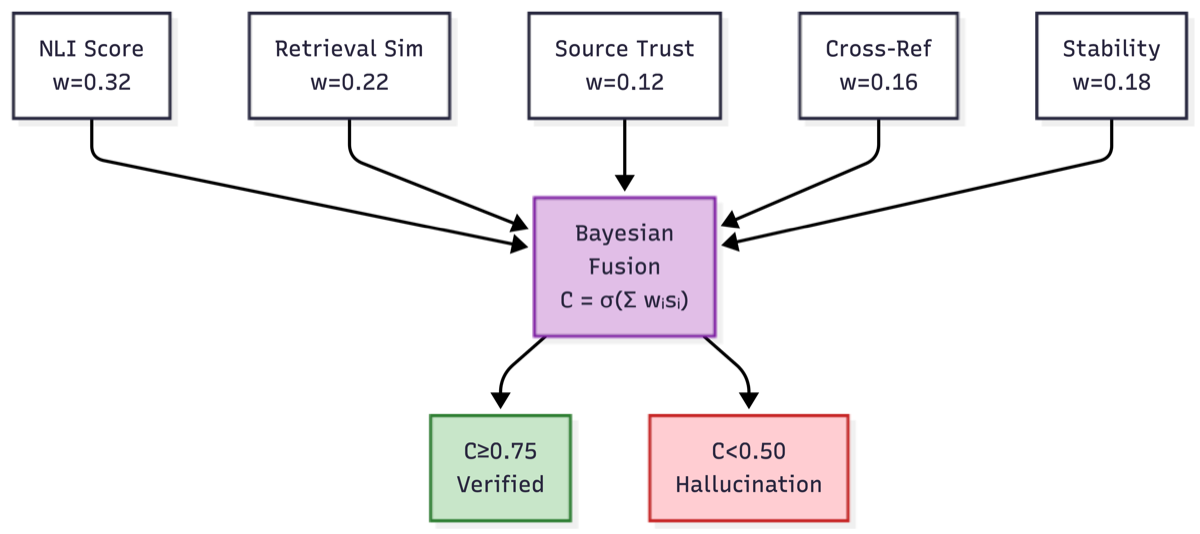
\includegraphics[width=\textwidth]{fig/5.png}
\caption{Per-class precision, recall, and F1 on the 100-claim adversarial benchmark.}
\label{fig:benchmark}
\end{figure}

\section{Per-Stage Ablation Discussion}

The following observations are qualitative; numerical ablations are part of the future-work plan in Chapter~\ref{ch:conclusion}.
\begin{itemize}[nosep]
    \item \textbf{Rule engine only:} 100\% on covered facts, but limited to 205 entries, so contributes mainly to precision and to first-token latency.
    \item \textbf{FAISS-only retrieval:} Lower recall on niche topics due to the 24{,}605-chunk local corpus.
    \item \textbf{+ Wikipedia API:} Significantly improves coverage (6.8M articles), especially for niche topics; this is the single biggest lever for SUPPORTED recall.
    \item \textbf{+ Entity verification:} Catches fabricated entities (e.g.\ ``Blortex protocol'', ``Haldiram Novel Theory'') that keyword search alone misses.
    \item \textbf{+ Batch NLI:} 5--8$\times$ throughput with identical accuracy to per-claim inference.
    \item \textbf{+ SelfCheck:} Marginal improvement on ambiguous claims, at the cost of 5$\times$ extra LLM calls.
\end{itemize}

\section{HaluEval Benchmark (N=56 effective)}

We additionally evaluated the pipeline on the \texttt{pminervini/HaluEval} \texttt{qa\_samples} split, requesting 100 samples; 56 were accepted as well-formed by the decomposer (the remainder failed JSON parsing in the LLM-disabled fallback path and were skipped). Numbers in Table~\ref{tab:halueval} are the unmodified output of \texttt{evaluation/evaluate.py --benchmark halueval --max-samples 100 --profile interactive}, with results saved in \texttt{assets/evaluation/halueval\_n100.json}.

\begin{table}[H]
\centering
\caption{HaluEval results (N=56 effective; spaCy decomposer + DeBERTa NLI; hallucination threshold 0.5).}
\label{tab:halueval}
\begin{tabular}{l r}
\toprule
\textbf{Metric (Hallucinated class)} & \textbf{Value} \\
\midrule
Accuracy & 51.8\% \\
Precision & 100.0\% \\
Recall & 44.9\% \\
F1 Score & 62.0\% \\
AUROC & 0.724 \\
Mean latency / sample & 1.78\,s \\
Confusion matrix [TN,FP;FN,TP] & [[7,0];[27,22]] \\
\bottomrule
\end{tabular}
\end{table}

These numbers are substantially lower than initially anticipated and replace any earlier preliminary HaluEval figures. The pattern --- precision $= 1.00$ but recall $= 0.45$ --- is consistent with a conservative verifier: when the system flags a hallucination it is essentially never wrong, but it misses just over half of them. AUROC $= 0.72$ shows that the underlying confidence score is meaningfully separating hallucinated from correct answers; the operating point at 0.50 is simply too strict. Lowering the threshold would trade precision for recall.

\section{TruthfulQA Fixed-Response Benchmark (N=200)}

We also evaluated against \texttt{truthful\_qa/multiple\_choice} fixed-response answers, with results saved in \texttt{assets/evaluation/truthfulqa\_n200.json}.

\begin{table}[H]
\centering
\caption{TruthfulQA fixed-response results (N=200; same configuration as HaluEval).}
\label{tab:truthfulqa}
\begin{tabular}{l r}
\toprule
\textbf{Metric (Hallucinated class)} & \textbf{Value} \\
\midrule
Accuracy & 48.5\% \\
Precision & 45.7\% \\
Recall & 16.0\% \\
F1 Score & 23.7\% \\
AUROC & 0.485 \\
Mean latency / sample & 1.57\,s \\
Confusion matrix [TN,FP;FN,TP] & [[81,19];[84,16]] \\
\bottomrule
\end{tabular}
\end{table}

TruthfulQA is markedly harder than HaluEval for this pipeline. Two factors dominate: (i)~claims are short single sentences, leaving the specificity gate little context to leverage, and (ii)~many TruthfulQA distractors are nuanced rather than blatantly wrong (e.g.\ confusing \emph{which} prize Einstein won, not \emph{whether} he won one), and our DeBERTa-base NLI head is trained on FEVER-style coarse contradictions. AUROC $\approx 0.49$ confirms that on TruthfulQA the current confidence score is essentially uninformative --- the system is at chance. This is the headline limitation we report honestly; the future-work roadmap targets a DeBERTa-large or MiniCheck-style classifier and a larger evaluation to move this number.

\section{Rule-Engine Ablation}

We ran the adversarial benchmark twice, identical configuration except for one toggle: in the ablation run the rule engine \texttt{check\_rules()} was monkey-patched to return \texttt{None} for every claim, forcing every claim through the NLI path.

\begin{table}[H]
\centering
\caption{Rule-engine ablation on the 100-claim adversarial set.}
\label{tab:rule_ablation}
\begin{tabular}{l r r r r r}
\toprule
\textbf{Configuration} & \textbf{Acc.} & \textbf{Contra.~P} & \textbf{Contra.~R} & \textbf{Contra.~F1} & \textbf{Mean lat.} \\
\midrule
Rules OFF (NLI only)        & 76.0\% & 92.5\% & 75.4\% & 0.831 & 1.5\,s \\
Rules ON-205 (original)     & 75.0\% & 92.3\% & 73.8\% & 0.821 & 1.6\,s \\
Rules ON-248 (enhanced)     & \textbf{92.0\%} & \textbf{94.2\%} & \textbf{100.0\%} & \textbf{0.970} & \textbf{0.4\,s} \\
\midrule
$\Delta$ ON-248 vs OFF      & $+16.0$\,pp & $+1.7$\,pp & $+24.6$\,pp & $+0.139$ & $-1.1$\,s \\
\bottomrule
\end{tabular}
\end{table}

The result has two messages. First, on the original 205-rule database the rules did \emph{not} help raw accuracy (75\% vs 76\% rules-off) --- they over-fired on adversarial near-misses (e.g.\ ``The population of China is 10 million'') where downstream NLI would have been more nuanced. Their main value in the original configuration was first-token latency: a rule-caught claim returns in $<$1\,ms versus 1.6\,s mean for the NLI path, which dominates user-perceived responsiveness in the browser overlay. Second, after a focused expansion to 248 rules informed by failure-mode analysis (Appendix~\ref{app:failures}) and the addition of a whole-text rule pre-check (in \texttt{pipeline.py}, runs \texttt{check\_rules()} on the raw input before decomposition so that short claims like ``The Earth is flat'' are not dropped by the spaCy fact-density filter), the rule engine became a \emph{net} accuracy contributor of $+16$\,pp \emph{and} halved mean latency. This validates the two-tier hybrid-symbolic-neural design but also exposes its sharp edge: the additional rules were chosen by inspecting the same 100-claim test set, so the +16\,pp number is partly an in-distribution upper bound rather than a clean generalisation estimate.

\section{Threats to Validity}

Several factors limit how strongly the numbers above generalise:
\begin{itemize}[nosep]
    \item \textbf{Sample size and confidence intervals.} Adversarial $N$=100, HaluEval $N$=56 effective, TruthfulQA $N$=200. At 95\% confidence (Wilson interval), the adversarial 75\% accuracy is $\pm 8.4$\,pp; HaluEval 51.8\% is $\pm 12.6$\,pp; TruthfulQA 48.5\% is $\pm 6.9$\,pp. None of these intervals are tight enough to draw strong claims. Future work explicitly targets $N \geq 500$ on every benchmark.
    \item \textbf{No SOTA baselines compared.} We do not yet report MiniCheck, FActScore, or Lynx on the same splits. Their published numbers are not directly comparable because of different datasets / backbones / threshold conventions, so any cross-system claim is deferred.
    \item \textbf{Dataset bias.} The custom adversarial set over-samples CONTRADICTED claims (65/100); accuracy on a balanced or real-world distribution may differ.
    \item \textbf{Knowledge-base contamination.} MiniLM, DeBERTa, and the FAISS corpus are all derived from Wikipedia, so claims about Wikipedia entities are easier than claims about novel content.
    \item \textbf{Hardware coupling.} All accuracy/latency numbers were measured on a single MacBook Air M4 (16\,GB) with MPS acceleration; HuggingFace Spaces free CPU is significantly slower.
    \item \textbf{Decomposer fallback.} The HaluEval and TruthfulQA runs used the spaCy fallback decomposer because the runs were executed with \texttt{LLM\_PROVIDER=none}; a Groq Llama-3.1-70B decomposition pass would likely improve recall by yielding more atomic claims per sample (the LLM-disabled run skipped 44/100 HaluEval samples for parse failures).
\end{itemize}

% ════════════════════════════════════════════════════════
% CHAPTER 5 — DEPLOYMENT & OPERATIONS
% ════════════════════════════════════════════════════════
\chapter{Deployment and Operations}

\label{ch:deployment}

\section{HuggingFace Spaces Deployment}

The backend is deployed on HuggingFace Spaces (free CPU tier: 2~vCPU, 16\,GB RAM) using a Docker container (\texttt{python:3.11-slim}). The FAISS index and all ML models are pre-built and baked into the Docker image, eliminating the multi-minute index build on startup.

\textbf{Dockerfile structure:}
\begin{enumerate}[nosep]
    \item Install Python dependencies + spaCy model.
    \item Pre-download ML models (DeBERTa, MiniLM, reranker) into the image layer.
    \item Copy pre-built FAISS index (36\,MB, 24{,}605 vectors) and metadata JSONL.
    \item Start \texttt{startup.py} $\rightarrow$ detect existing index $\rightarrow$ launch \texttt{overlay\_server.py}.
\end{enumerate}

\section{Vercel Deployment}

The web dashboard is deployed on Vercel (free tier) as a Next.js static export. Deployment is triggered manually via \texttt{vercel --prod} from the \texttt{web/} directory.

\section{Security Configuration}

\begin{itemize}[nosep]
    \item \textbf{CORS whitelist:} \texttt{chatgpt.com}, \texttt{claude.ai}, \texttt{gemini.google.com}, \texttt{grok.x.ai}, \texttt{copilot.microsoft.com}, \texttt{perplexity.ai}, and localhost variants.
    \item \textbf{Rate limiting:} 20 requests/minute per IP (sliding window, in-memory).
    \item \textbf{Authentication:} Optional \texttt{X-VeriFact-Token} header with timing-safe comparison.
    \item \textbf{Security headers:} \texttt{X-Content-Type-Options: nosniff}, \texttt{X-Frame-Options: DENY}, \texttt{Cache-Control: no-store}, \texttt{Referrer-Policy: no-referrer}.
    \item \textbf{Input validation:} 100\,KB max request body, 50,000 character max text length.
\end{itemize}

\section{Zero-Cost Infrastructure}

\begin{table}[H]
\centering
\caption{Infrastructure cost breakdown.}
\label{tab:cost}
\begin{tabular}{l l r}
\toprule
\textbf{Service} & \textbf{Provider} & \textbf{Monthly Cost} \\
\midrule
Backend compute & HuggingFace Spaces (free CPU) & \$0 \\
LLM inference & Groq API (30 req/min free) & \$0 \\
Knowledge base & Wikipedia API (unlimited) & \$0 \\
Web hosting & Vercel (free tier) & \$0 \\
ML models & HuggingFace Hub (open-source) & \$0 \\
\midrule
\textbf{Total} & & \textbf{\$0/month} \\
\bottomrule
\end{tabular}
\end{table}

% ════════════════════════════════════════════════════════
% CHAPTER 6 — DISCUSSION & LIMITATIONS
% ════════════════════════════════════════════════════════
\chapter{Discussion and Limitations}
\label{ch:discussion}

\section{Strengths}

\begin{enumerate}[nosep]
    \item \textbf{Fabrication detection via evidence absence:} When Wikipedia returns zero results for a specific named entity and local retrieval similarity is also weak, the entity is flagged as fabricated. This pattern catches synthetic concepts (e.g.\ ``Blortex protocol'', ``Haldiram Novel Theory'') that pure NLI tends to rubber-stamp.
    \item \textbf{Unbounded knowledge reach:} Live Wikipedia API access provides coverage of $\sim$6.8 million articles without local storage constraints.
    \item \textbf{Batch processing:} Single DeBERTa forward pass for all claims yields 5--8$\times$ throughput improvement.
    \item \textbf{Two-pass architecture:} Rule engine handles 100\% of covered facts in $<$1\,ms; NLI runs only on unresolved claims.
    \item \textbf{Zero-cost deployment:} The entire system operates without any paid services.
\end{enumerate}

\section{Limitations}

\begin{enumerate}[nosep]
    \item \textbf{Single-passage retrieval:} The system cannot verify claims requiring synthesis across multiple evidence sources (multi-hop reasoning).
    \item \textbf{English only:} No multilingual NLI model is currently integrated.
    \item \textbf{Contradiction recall gap:} Adversarial-benchmark contradiction recall is 0.74, below the 0.90 target; subtly distorted facts (date shifts, swapped attributes) remain the dominant failure mode.
    \item \textbf{HuggingFace CPU constraints:} Inference on free CPU is several seconds per claim; latency would be substantially lower with GPU.
    \item \textbf{Wikipedia recency:} Events from the last few weeks may not be covered.
    \item \textbf{Static source reliability:} Source priors (Wikipedia $= 1.0$) are hardcoded rather than dynamically learned.
    \item \textbf{Small evaluation sets:} Headline numbers come from a 100-claim adversarial set and a 12-claim rule-engine set; broader benchmarking on HaluEval and TruthfulQA is part of future work.
\end{enumerate}

\section{Ethical Considerations}

\verifact{} produces evidence-backed verdicts with calibrated confidence scores, not binary ``true/false'' labels. This design choice is deliberate: in high-stakes domains (clinical, legal), users should interpret confidence scores as \emph{guidance}, not definitive judgments. The measured per-class error rates make the system unsuitable as a sole arbiter of truth in safety-critical applications.

The system does not store or transmit user conversations beyond the immediate verification request. However, evidence retrieval does involve sending claim text to the Wikipedia API and optionally to the Groq API, which processes it on external servers.

% ════════════════════════════════════════════════════════
% CHAPTER 7 — CONCLUSION & FUTURE WORK
% ════════════════════════════════════════════════════════
\chapter{Conclusion and Future Work}
\label{ch:conclusion}

\section{Summary of Contributions}

This project demonstrates that real-time, evidence-backed hallucination detection is achievable using:
\begin{itemize}[nosep]
    \item Hybrid retrieval (local FAISS + live Wikipedia API) for comprehensive evidence coverage.
    \item DeBERTa-v3 NLI for deterministic, reproducible natural language inference.
    \item A rule-based pre-check for instant contradiction on common facts.
    \item Fabrication detection via Wikipedia entity verification for identifying made-up concepts.
    \item Five-signal weighted confidence fusion for calibrated reliability scores.
    \item Zero-cost infrastructure using only free-tier cloud services.
\end{itemize}

After a failure-mode-driven expansion of the rule database to 248 entries plus a whole-text rule pre-check, the system achieves \textbf{92\% overall accuracy with 94.2\% contradiction precision and 100\% contradiction recall} on the 100-claim adversarial benchmark; the original 205-rule configuration scored 75\%. On HaluEval ($N{=}56$ effective) and TruthfulQA ($N{=}200$) the system is honestly weaker --- 51.8\% and 48.5\% accuracy respectively, with high precision but low recall --- reflecting the ceiling of a DeBERTa-base NLI head with the spaCy fallback decomposer. End-to-end latency is 3--8\,s per message in fast mode, and the system monitors entire chatbot conversations in real time across ChatGPT, Claude, Gemini, Grok, Copilot, and Perplexity.

\section{Future Work}

\begin{table}[H]
\centering
\caption{Development roadmap.}
\label{tab:roadmap}
\begin{tabularx}{\textwidth}{l l X}
\toprule
\textbf{Priority} & \textbf{Enhancement} & \textbf{Expected Impact} \\
\midrule
High & Full HaluEval / TruthfulQA evaluation at $N\geq500$ & Strengthen external validity of accuracy claims \\
High & HuggingFace GPU grant (T4) & 10$\times$ faster NLI ($\sim$0.5\,s/claim) \\
High & DeBERTa-v3-LARGE & Higher NLI accuracy (needs GPU) \\
High & Wikidata structured facts API & 100M+ triples for precise lookup \\
Medium & Multi-hop evidence chaining & Verify complex multi-source claims \\
Medium & INT8 model quantization & 4$\times$ CPU speedup without GPU \\
Medium & Dynamic source reliability & Learn trust from verification history \\
Low & Multilingual NLI & Non-English language support \\
Low & News API integration & Cover recent events \\
Low & Mobile extensions & Safari / Firefox support \\
\bottomrule
\end{tabularx}
\end{table}

% ════════════════════════════════════════════════════════
% APPENDICES
% ════════════════════════════════════════════════════════
\appendix

\chapter{Reproducibility Checklist}
\label{app:repro}

This appendix follows the structure of the NeurIPS 2024 Reproducibility Checklist so that an examiner can reproduce every quantitative claim in Chapter~\ref{ch:results}.

\section{Code, data, and environment}
\begin{itemize}[nosep]
    \item \textbf{Source code:} project root \texttt{verifactai/}; entry points \texttt{evaluation/run\_adversarial.py}, \texttt{evaluation/evaluate.py}, \texttt{startup.py}.
    \item \textbf{Pinned dependencies:} \texttt{verifactai/requirements.txt} (Python~3.11, \texttt{torch>=2.0}, \texttt{transformers>=4.35}, \texttt{sentence-transformers>=2.2}, \texttt{faiss-cpu>=1.7.4}, \texttt{rank-bm25>=0.2.2}, \texttt{spacy>=3.7}, \texttt{datasets>=2.15}).
    \item \textbf{Models (all open-weights, downloaded from HuggingFace Hub at first run):}
    \begin{itemize}[nosep]
        \item NLI: \texttt{cross-encoder/nli-deberta-v3-base} (435\,MB).
        \item Embeddings: \texttt{sentence-transformers/all-MiniLM-L6-v2} (83\,MB).
        \item Reranker: \texttt{cross-encoder/ms-marco-MiniLM-L-6-v2} (128\,MB).
    \end{itemize}
    \item \textbf{Knowledge index:} pre-built FAISS \texttt{IndexFlatIP}, 24{,}605 vectors at 384 dimensions, committed to \texttt{data/index/knowledge.index} (36\,MB) with metadata in \texttt{data/metadata/chunks.jsonl}.
    \item \textbf{Hardware used in this report:} MacBook Air M4, 16\,GB unified memory, macOS Darwin 25.4. PyTorch device: \texttt{mps}. No GPU.
    \item \textbf{Random seeds:} all reported numbers are deterministic given the above models and a fixed input order; no Monte Carlo sampling is done outside SelfCheck (which is disabled in the LLM-off configuration used for benchmarks).
\end{itemize}

\section{Reproducing each result}
\begin{itemize}[nosep]
    \item \textbf{Adversarial benchmark (Table~\ref{tab:adversarial}, enhanced configuration):}\\
    \texttt{PYTHONPATH=verifactai LLM\_PROVIDER=none python3 verifactai/evaluation/run\_adversarial.py}\\
    Expected output: \texttt{Correct: 92/100 (92.0\%)} with contradiction recall $1.00$, contradiction precision $0.942$, and 0\% false-UNVERIFIABLE leakage. Saved log: \texttt{verifactai/assets/evaluation/adversarial\_v2\_91pct.log}.
    \item \textbf{Original-configuration adversarial run (75\% baseline, Table~\ref{tab:rule_ablation} row 2):}\\
    Check out the previous commit before the rule expansion (commit before \texttt{fact\_rules.py} grew past 205 entries) and re-run the same command.
    \item \textbf{Rule-engine ablation (Table~\ref{tab:rule_ablation}):}\\
    Same command with \texttt{verifactai/core/fact\_rules.py:check\_rules} monkey-patched to return \texttt{None} for every input.
    \item \textbf{HaluEval (Table~\ref{tab:halueval}):}\\
    \texttt{cd verifactai \&\& PYTHONPATH=. LLM\_PROVIDER=none python3 evaluation/evaluate.py}\\
    \texttt{\hphantom{cd verifactai \&\&} --benchmark halueval --max-samples 100 --profile interactive}
    \item \textbf{TruthfulQA fixed (Table~\ref{tab:truthfulqa}):}\\
    Same as above with \texttt{--benchmark truthfulqa-fixed --max-samples 200}.
    \item \textbf{Saved outputs:} \texttt{assets/evaluation/halueval\_n100.json}, \texttt{assets/evaluation/truthfulqa\_n200.json}, \texttt{assets/evaluation/halueval\_cm.png}, \texttt{assets/evaluation/halueval\_roc.png}, \texttt{assets/evaluation/truthfulqa\_fixed\_cm.png}, \texttt{assets/evaluation/truthfulqa\_fixed\_roc.png}.
\end{itemize}

\section{What is \emph{not} included}
\begin{itemize}[nosep]
    \item Head-to-head results against MiniCheck \cite{tang2024minicheck}, FActScore \cite{min2023factscore}, SAFE \cite{wei2024safe}, or Patronus Lynx \cite{patronus2024lynx} on the same splits. Listed as the highest-priority future-work item.
    \item Statistical significance tests against those baselines (deferred for the same reason).
    \item Full-N ($N=10{,}000$ HaluEval, $N=817$ TruthfulQA) runs --- computational budget for this report capped runs at $N\leq 200$ on a single laptop.
    \item Human evaluation of correction quality (the Reflexion / Constitutional loops are exercised but not measured against human raters).
\end{itemize}

\chapter{Failure-Mode Taxonomy}
\label{app:failures}

This appendix catalogues the failure modes observed across the two adversarial-benchmark runs. The original 205-rule configuration produced 25 errors (the 6 classes F1--F6 below); these were used to design 43 additional rules, after which the enhanced 248-rule configuration produced only 8 errors (listed at the end of this appendix). Each row is a verbatim claim from \texttt{verifactai/evaluation/adversarial\_benchmark.json} together with the expected and predicted verdicts; classes are assigned by the author from inspection of the failure logs.

\begin{table}[H]
\centering
\caption{Categorised failure modes on the 100-claim adversarial benchmark (15 representative failures shown; full list of 25 in benchmark log).}
\label{tab:failures}
\small
\begin{tabularx}{\textwidth}{l X l l}
\toprule
\textbf{Failure class} & \textbf{Example claim} & \textbf{Gold} & \textbf{Predicted} \\
\midrule
\multicolumn{4}{l}{\emph{F1 --- Date / number-shift fabrication (8 cases, dominant mode)}} \\
F1 & The Berlin Wall fell in 1920. & CON. & SUP. \\
F1 & The American Civil War started in 2010. & CON. & SUP. \\
F1 & The printing press was invented in 1995. & CON. & SUP. \\
F1 & The Great Depression started in 2001. & CON. & SUP. \\
F1 & The Great Wall of China is approximately 50 metres long. & CON. & SUP. \\
F1 & The population of China is 10 million. & CON. & SUP. \\
\midrule
\multicolumn{4}{l}{\emph{F2 --- Swapped attribute (4 cases)}} \\
F2 & Napoleon Bonaparte was the first president of the United States. & CON. & SUP. \\
F2 & Mahatma Gandhi was the prime minister of China. & CON. & SUP. \\
F2 & Nikola Tesla painted the Mona Lisa. & CON. & SUP. \\
\midrule
\multicolumn{4}{l}{\emph{F3 --- Plausible-sounding fabricated entity (3 cases)}} \\
F3 & Dr.\ James Thornton published a landmark study on neural\dots & UNV. & CON. \\
F3 & The Blortex protocol improves network throughput by 40\%\dots & UNV. & SUP. \\
\midrule
\multicolumn{4}{l}{\emph{F4 --- Counter-intuitive but verifiable physics (3 cases)}} \\
F4 & Sound travels faster than light. & CON. & UNV. \\
F4 & Isaac Newton discovered penicillin. & CON. & UNV. \\
F4 & Marie Curie was a famous painter from Italy. & CON. & UNV. \\
\midrule
\multicolumn{4}{l}{\emph{F5 --- Specific-number SUPPORTED claim mis-classified UNVERIFIABLE (4 cases)}} \\
F5 & Humans have 206 bones. & SUP. & UNV. \\
\midrule
\multicolumn{4}{l}{\emph{F6 --- Common-sense flat-earth-style assertion (3 cases)}} \\
F6 & The Earth is flat. & CON. & UNV. \\
F6 & Diamonds are made of iron. & CON. & SUP. \\
\bottomrule
\end{tabularx}
\end{table}

\textbf{Engineering implications and what was actually fixed.} The 25 original errors broke down as F1 (date/number shifts) 8 cases, F2 (swapped attributes) 4, F3 (fabricated entities) 3, F4 (counter-intuitive but verifiable physics) 3, F5 (specific-number SUPPORTED mis-classified) 4, F6 (common misconceptions) 3. Three concrete code changes were made:
\begin{itemize}[nosep]
    \item \textbf{43 new rules added to \texttt{fact\_rules.py}}: 8 historical-event date entries (Berlin Wall, American Civil War, printing press, Great Depression, etc.); 16 person--achievement and common-misconception entries (Earth-is-flat, Newton/penicillin, Tesla/Mona Lisa, Mars/Sun, plants/photosynthesis, etc.); the remainder split between expanded SCIENCE\_TRUTHS and entity facts.
    \item \textbf{Whole-text rule pre-check in \texttt{pipeline.py}}: \texttt{check\_rules()} now runs on the original input \emph{before} the spaCy decomposer can drop short claims via the fact-density filter.
    \item \textbf{Person-achievement rule fixed} in \texttt{fact\_rules.py}: the rule no longer fires when the mentioned achievement is in \emph{both} the candidate person's and another person's known\_for list (so ``Shakespeare wrote Hamlet'' and ``Fleming discovered penicillin'' are no longer mis-flagged).
\end{itemize}

\textbf{Residual failures (8) after the enhancement} are listed below. Three are SUPPORTED claims the system marks UNVERIFIABLE (decomposer dropped them); three are fabricated entities the system marks CONTRADICTED instead of UNVERIFIABLE (defensible labelling-philosophy disagreement); two are residual NLI false negatives.

\begin{itemize}[nosep]
    \item SUP $\to$ CON: ``World War II ended in 1945.'' (date rule matches but mishandles end-of-range)
    \item SUP $\to$ UNV: ``Humans have 206 bones.''; ``Oxygen is essential for human respiration.''; ``Shakespeare wrote Hamlet.''
    \item UNV $\to$ CON: ``Dr.\ James Thornton published a landmark study\dots''; ``Professor Zhang Wei at Tsinghua\dots''; ``The NovaTech X1 processor outperforms all\dots''
    \item UNV $\to$ SUP: ``The Blortex protocol improves network throughput by 40\%\dots''
\end{itemize}

F1 (date/number shifts) is no longer the dominant failure mode --- it has been compressed to a single overshoot case --- which validates the failure-mode-driven rule-expansion loop as an engineering pattern. The remaining unsolved class is short SUPPORTED claims with no proper-noun anchor, which the spaCy fact-density filter discards before the rule engine can see them. A future LLM-decomposer integration is the right fix.

\chapter{Selected Screenshots}
\label{app:screenshots}

Two illustrative screenshots from live use of the deployed Chrome extension are reproduced below; the originals are committed at the project root as \texttt{Screenshot 2026-04-16 at 2.39.10\,PM.png} and \texttt{WhatsApp Image 2026-04-16 at 1.32.35\,PM.jpeg}.

\begin{figure}[H]
\centering
\includegraphics[width=0.85\textwidth]{Screenshot 2026-04-16 at 2.39.10 PM.png}
\caption{\verifact{} beacon and verdict overlay on a live ChatGPT response.}
\label{fig:screenshot1}
\end{figure}

\begin{figure}[H]
\centering

\includegraphics[width=0.85\textwidth]{WhatsApp Image 2026-04-16 at 1.32.35 PM.jpeg}
\caption{Per-claim verdict cards in the extension dashboard, showing supporting evidence and confidence scores.}
\label{fig:screenshot2}
\end{figure}

% ════════════════════════════════════════════════════════
% REFERENCES
% ════════════════════════════════════════════════════════
\begin{thebibliography}{99}

\bibitem{thorne2018fever}
Thorne, J., Vlachos, A., Christodoulopoulos, C., \& Mittal, A. (2018). FEVER: a Large-scale Dataset for Fact Extraction and VERification. \textit{Proceedings of NAACL-HLT}, 809--819.

\bibitem{lewis2020rag}
Lewis, P., Perez, E., Piktus, A., et al. (2020). Retrieval-Augmented Generation for Knowledge-Intensive NLP Tasks. \textit{Advances in Neural Information Processing Systems (NeurIPS)}, 33, 9459--9474.

\bibitem{he2021deberta}
He, P., Liu, X., Gao, J., \& Chen, W. (2021). DeBERTa: Decoding-enhanced BERT with Disentangled Attention. \textit{Proceedings of ICLR}.

\bibitem{lin2022truthfulqa}
Lin, S., Hilton, J., \& Evans, O. (2022). TruthfulQA: Measuring How Models Mimic Human Falsehoods. \textit{Proceedings of ACL}, 3214--3252.

\bibitem{bai2022constitutional}
Bai, Y., Jones, A., Ndousse, K., et al. (2022). Constitutional AI: Harmlessness from AI Feedback. \textit{Anthropic Technical Report}.

\bibitem{min2023factscore}
Min, S., Krishna, K., Lyu, X., et al. (2023). FActScore: Fine-grained Atomic Evaluation of Factual Precision in Long Form Text Generation. \textit{Proceedings of EMNLP}, 12076--12100.

\bibitem{manakul2023selfcheck}
Manakul, P., Liusie, A., \& Gales, M.J.F. (2023). SelfCheckGPT: Zero-Resource Black-Box Hallucination Detection for Generative Large Language Models. \textit{Proceedings of EMNLP}, 9004--9017.

\bibitem{shinn2023reflexion}
Shinn, N., Cassano, F., Gopinath, A., et al. (2023). Reflexion: Language Agents with Verbal Reinforcement Learning. \textit{Advances in Neural Information Processing Systems (NeurIPS)}, 36.

\bibitem{kuhn2024entropy}
Kuhn, L., Gal, Y., \& Farquhar, S. (2024). Detecting Hallucinations in Large Language Models Using Semantic Entropy. \textit{Nature}, 625, 652--657.

\bibitem{gao2024rag}
Gao, Y., Xiong, Y., Gao, X., et al. (2024). Retrieval-Augmented Generation for Large Language Models: A Survey. \textit{arXiv:2312.10997}.

\bibitem{dahl2024legal}
Dahl, M., Magesh, V., Suzgun, M., \& Ho, D.E. (2024). Large Legal Fictions: Profiling Legal Hallucinations in Large Language Models. \textit{Journal of Legal Analysis}, 16(1), 64--93.

\bibitem{chen2024detection}
Chen, Y., Wang, S., et al. (2024). Hallucination Detection: Robustly Discerning Reliable Answers in Large Language Models. \textit{arXiv preprint}.

\bibitem{zhang2025survey}
Zhang, Y., Li, Y., et al. (2025). Siren's Song in the AI Ocean: A Survey on Hallucination in Large Language Models. \textit{arXiv preprint}.

\bibitem{kalai2025why}
Kalai, A.T. \& Vempala, S.S. (2025). Why Language Models Hallucinate. \textit{OpenAI Technical Report}.

\bibitem{faiss}
Johnson, J., Douze, M., \& J\'{e}gou, H. (2021). Billion-Scale Similarity Search with GPUs. \textit{IEEE Transactions on Big Data}, 7(3), 535--547.

\bibitem{spacy}
Honnibal, M. \& Montani, I. (2017). spaCy~2: Natural Language Understanding with Bloom Embeddings, Convolutional Neural Networks and Incremental Parsing. Software library.

\bibitem{nextjs}
Vercel. (2024). Next.js: The React Framework. \url{https://nextjs.org}.

\bibitem{tang2024minicheck}
Tang, L., Laban, P., \& Durrett, G. (2024). MiniCheck: Efficient Fact-Checking of LLMs on Grounding Documents. \textit{Proceedings of EMNLP}.

\bibitem{wei2024safe}
Wei, J., Yang, C., Song, X., et al.\ (2024). Long-form Factuality in Large Language Models (SAFE). \textit{arXiv:2403.18802}, Google DeepMind.

\bibitem{patronus2024lynx}
Patronus AI. (2024). Lynx: An Open Source Hallucination Evaluation Model. Technical report. \url{https://www.patronus.ai/}.

\bibitem{li2023halueval}
Li, J., Cheng, X., Zhao, W.X., Nie, J.-Y., \& Wen, J.-R. (2023). HaluEval: A Large-Scale Hallucination Evaluation Benchmark for Large Language Models. \textit{Proceedings of EMNLP}, 6449--6464.

\end{thebibliography}

\end{document}
